% \iffalse meta-comment
% !TEX program  = LuaLaTeX
%
% hustreport.dtx
%
% Copyright (C) 2013-2014 by Xu Cheng <xucheng@me.com>
%               2014-2016 by hust-latex <https://github.com/hust-latex>
%
% This work may be distributed and/or modified under the
% conditions of the LaTeX Project Public License, either version 1.3
% of this license or (at your option) any later version.
% The latest version of this license is in
%   http://www.latex-project.org/lppl.txt
% and version 1.3 or later is part of all distributions of LaTeX
% version 2005/12/01 or later.
%
% This work has the LPPL maintenance status `maintained'.
%
% The Current Maintainer of this work is hust-latex Organization.
%
% This work consists of the files hustreport.dtx,
% hustreport.ins and the derived file hustreport.cls
% along with its document and example files.
%
% \fi
%
% \iffalse
%<*driver>
\ProvidesFile{hustreport.dtx}
%</driver>
%<class>\NeedsTeXFormat{LaTeX2e}[1999/12/01]
%<class>\ProvidesClass{hustreport}
%<*class>
[2016/06/01 v1.1 A Report Template for Huazhong University of Science and Technology]
%</class>
%
%<*driver>
\documentclass[12pt,a4paper,numbered,full]{l3doc}

\usepackage{fontspec}
\setmainfont[Ligatures={Common,TeX}]{Tex Gyre Pagella}
\setsansfont[Ligatures={Common,TeX}]{Droid Sans}
\setmonofont{CMU Typewriter Text}
\defaultfontfeatures{Mapping=tex-text,Scale=MatchLowercase}

\usepackage{luatexja-fontspec}
\setmainjfont[BoldFont={AdobeHeitiStd-Regular},ItalicFont={AdobeKaitiStd-Regular}]{AdobeSongStd-Light}
\setsansjfont{AdobeKaitiStd-Regular}
\defaultjfontfeatures{JFM=kaiming}
\newjfontfamily\KAI{AdobeKaitiStd-Regular}
\newjfontfamily\FANGSONG{AdobeFangsongStd-Regular}

\linespread{1.2}\selectfont

\usepackage[top=1.2in,bottom=1.2in,left=1.5in,right=1in]{geometry}
\pagewidth=\paperwidth
\pageheight=\paperheight

\usepackage{color}
\usepackage[table]{xcolor}

\definecolor{hyperreflinkred}{RGB}{128,23,31}
\hypersetup{
  unicode,
  bookmarksnumbered=true,
  bookmarksopen=true,
  bookmarksopenlevel=0,
  breaklinks=true,
  colorlinks=true,
  allcolors=hyperreflinkred,
  linktoc=page,
  plainpages=false,
  pdfpagelabels=true,
  pdfstartview={XYZ null null 1}
}
\usepackage{indentfirst}
\setlength{\parindent}{2em}

\usepackage{titlesec,titletoc}
\usepackage[titles]{tocloft}
\setcounter{tocdepth}{2}
\setcounter{secnumdepth}{3}

\usepackage{enumitem}
\setlist{noitemsep,partopsep=0pt,topsep=.8ex}
\setlist[1]{labelindent=\parindent}
\setlist[enumerate,1]{label=\arabic*.,ref=\arabic*}
\setlist[enumerate,2]{label*=\arabic*,ref=\theenumi.\arabic*}
\setlist[enumerate,3]{label=\emph{\alph*}),ref=\theenumii\emph{\alph*}}

\usepackage{listings}
\definecolor{lstgreen}{rgb}{0,0.6,0}
\definecolor{lstgray}{rgb}{0.5,0.5,0.5}
\definecolor{lstmauve}{rgb}{0.58,0,0.82}
\lstset{
  basicstyle=\footnotesize\ttfamily\FANGSONG,
  keywordstyle=\color{blue}\bfseries,
  commentstyle=\color{lstgreen}\itshape\KAI,
  stringstyle=\color{lstmauve},
  showspaces=false,
  showstringspaces=false,
  showtabs=false,
  numbers=left,
  numberstyle=\tiny\color{lstgray},
  frame=lines,
  rulecolor=\color{black},
  breaklines=true
}

\AtBeginEnvironment{verbatim}{\small}
\let\AltMacroFont\MacroFont

\usepackage{metalogo}
\usepackage{notes}
\usepackage{tabularx}

\newcommand{\tabincell}[2]{\begin{tabular}{@{}#1@{}}#2\end{tabular}}

\renewcommand{\cftsecleader}{\cftdotfill{\cftdotsep}}
\setlength{\cftsecindent}{2em}
\setlength{\cftsubsecindent}{4em}
\makeatletter
\newskip\HUST@oldcftbeforepartskip
\HUST@oldcftbeforepartskip=\cftbeforepartskip
\newskip\HUST@oldcftbeforesecskip
\HUST@oldcftbeforesecskip=\cftbeforesecskip
\let\HUST@oldl@part\l@part
\let\HUST@oldl@section\l@section
\let\HUST@oldl@subsection\l@subsection
\def\l@part#1#2{\HUST@oldl@part{#1}{#2}\cftbeforepartskip=3pt}
\def\l@section#1#2{\HUST@oldl@section{#1}{#2}\cftbeforepartskip=\HUST@oldcftbeforepartskip\cftbeforesecskip=3pt}
\def\l@subsection#1#2{\HUST@oldl@subsection{#1}{#2}\cftbeforesecskip=\HUST@oldcftbeforesecskip}
\makeatother

\titleformat{\part}
  {
    \bfseries
    \centering
    \fontsize{18pt}{23.4pt}\selectfont
  }
  {\thepart}
  {1em}
  {}
\let\oldpart\part
\def\part#1{\newpage\oldpart{#1}}

\def\orvar{\textnormal{|}}

\IndexPrologue
 {
  \part{Index}
  The~italic~numbers~denote~the~pages~where~the~
  corresponding~entry~is~described,~
  numbers~underlined~point~to~the~definition,~
  all~others~indicate~the~places~where~it~is~used.
 }

\EnableCrossrefs
\CodelineIndex
\RecordChanges

\def\email#1{
  \href{mailto:#1}{\texttt{#1}}
}

\usepackage{xparse}
\ExplSyntaxOn
\DeclareDocumentCommand\pkgurl{o m}
{
    \IfNoValueTF{#1}
    {
        \href
        {
        http://mirrors.ctan.org/help/Catalogue/entries/
        \str_fold_case:n {#2} .html
        }
        { \textsf{#2} }
    }
    {
        \href
        {
        http://mirrors.ctan.org/help/Catalogue/entries/
        \str_fold_case:n {#1} .html
        }
        { \textsf{#2} }
    }
}
\ExplSyntaxOff

\begin{document}
\DocInput{hustreport.dtx}
\end{document}
%</driver>
% \fi
%
% \CheckSum{1482}
%
% \iffalse
%<*!(example-bib)>
% \fi
%% \CharacterTable
%% {Upper-case    \A\B\C\D\E\F\G\H\I\J\K\L\M\N\O\P\Q\R\S\T\U\V\W\X\Y\Z
%%  Lower-case    \a\b\c\d\e\f\g\h\i\j\k\l\m\n\o\p\q\r\s\t\u\v\w\x\y\z
%%  Digits        \0\1\2\3\4\5\6\7\8\9
%%  Exclamation   \!     Double quote  \"     Hash (number) \#
%%  Dollar        \$     Percent       \%     Ampersand     \&
%%  Acute accent  \'     Left paren    \(     Right paren   \)
%%  Asterisk      \*     Plus          \+     Comma         \,
%%  Minus         \-     Point         \.     Solidus       \/
%%  Colon         \:     Semicolon     \;     Less than     \<
%%  Equals        \=     Greater than  \>     Question mark \?
%%  Commercial at \@     Left bracket  \[     Backslash     \\
%%  Right bracket \]     Circumflex    \^     Underscore    \_
%%  Grave accent  \`     Left brace    \{     Vertical bar  \|
%%  Right brace   \}     Tilde         \~}
% \iffalse
%</!(example-bib)>
% \fi
%
% \changes{v1.0}{2013/07/01}{Initial version}
% \changes{v1.1}{2016/06/01}{Fix for TeXLive 2016. Remove \texttt{interfaces} and other problematic package}
% \changes{v1.2}{2016/07/05}{Fix for \XeLaTeX}
%
% \GetFileInfo{hustreport.dtx}
%
% \DoNotIndex{\#,\$,\%,\&,\@,\\,\{,\},\^,\_,\~,\ ,\,}
% \DoNotIndex{\def,\if,\else,\fi,\gdef,\long,\let}
% \DoNotIndex{\@ne,\@nil}
% \DoNotIndex{\begingroup,\endgroup,\advance}
% \DoNotIndex{\newcommand,\renewcommand}
% \DoNotIndex{\newenvironment,\renewenvironment}
% \DoNotIndex{\RequirePackage}
%
% \title{A Report Template for Huazhong University of Science and Technology: the \textsf{hustreport} class
% \thanks{This document corresponds to \textsf{hustreport.cls}~\fileversion, dated \filedate.}}
% \author{Xu Cheng \\ \email{xucheng@me.com}}
% \date{\today}
%
% \begingroup
% \hypersetup{allcolors=black}
% \maketitle
% \endgroup
% \tableofcontents
%
% \part{Introduction}
%
% This is a report template for \href{http://www.hust.edu.cn/}{Huazhong University of Science \& Technology}. This template is distributed in the hope that it will be useful, but WITHOUT ANY WARRANTY; without even the implied warranty of MERCHANTABILITY or FITNESS FOR A PARTICULAR PURPOSE.
%
% The whole project is published under LPPL v1.3 License at \href{https://github.com/hust-latex/hustreport}{GitHub}.
%
% 中文使用说明见\autoref{part:中文使用说明}。
%
% English version instruction is in \autoref{part:English Version Instruction}.
%
% \part{中文使用说明}\label{part:中文使用说明}
%
% \section{使用必要条件}
%
% \begin{enumerate}
%     \item 安装最新版本的\href{http://www.tug.org/texlive/}{\texttt{TeXLive}}(推荐)或\href{http://miktex.org/}{\texttt{MiKTeX}}。因为未及时更新的宏包可能存在未修复的bug,请确保所有宏包都更新至最新。
%     \item 安装如下中文字体\footnote{本模板所用到的英文字体\textsf{Tex Gyre Termes},\textsf{Droid Sans}和\textsf{CMU Typewriter Text}均默认安装于\textsf{TeXLive}和\textsf{MiKTeX}中。}:
%     \begin{enumerate}[label=\emph{\alph*})]
%         \item \textsf{AdobeSongStd-Light}
%         \item \textsf{AdobeKaitiStd-Regular}
%         \item \textsf{AdobeHeitiStd-Regular}
%         \item \textsf{AdobeFangsongStd-Regular}
%     \end{enumerate}
%     \begin{informationnote}
%     如果使用\textnormal{\LuaTeX},安装字体之后需运行命令\verb+mkluatexfontdb+生成字体索引。
%     \end{informationnote}
% \end{enumerate}
%
% \section{安装}
%
% \subsection{安装到本地}
%
% 使用如下命令即可安装本模板到本地:
% \begin{verbatim}
%     make install
% \end{verbatim}
% 如需卸载,则使用如下命令:
% \begin{verbatim}
%     make uninstall
% \end{verbatim}
%
% 对于没有安装\verb+Make+的Windows系统用户,可以使用如下命令安装:
% \begin{verbatim}
%     makewin32.bat install
% \end{verbatim}
% 如需卸载,则使用如下命令:
% \begin{verbatim}
%     makewin32.bat uninstall
% \end{verbatim}
% 虽然\verb+makewin32.bat+表现与\verb+Makefile+极其相似,但是还是强烈建议你安装\verb+Make+,对于Windows用户可以在\href{http://gnuwin32.sourceforge.net/packages/make.htm}{这里}下载。
%
% \subsection{免安装使用}
%
% 如果你希望临时使用本模板,而非安装到本地供长期使用。使用如下命令解压模板文件:
% \begin{verbatim}
%     make unpack
% \end{verbatim}
% 对于没有安装\verb+Make+的Windows系统用户,则使用如下命令解压:
% \begin{verbatim}
%     makewin32.bat unpack
% \end{verbatim}
%
% 再将\verb+hustreport+目录下的如下文件拷贝到你\TeX{}工程根目录下即可:
% \begin{itemize}
%     \item \verb+hustreport.cls+
%     \item \verb+hust-title.eps+
%     \item \verb+hust-title.pdf+
% \end{itemize}
%
% \section{基本用法}
%
% \begin{importantnote}
% 本文档只能使用\textnormal{\XeLaTeX}或\textnormal{\LuaLaTeX}(推荐)编译。
% \end{importantnote}
%
% 在源文件开头处选择加载本文档类型,即可使用本模板,如下所示:
% \begin{verbatim}
%     \documentclass[language=chinese]{hustreport}
% \end{verbatim}
%
% \subsection{文档类型选项}
%
% 加载本文档类型时,有如下三个选项提供选择。
%
% \begin{function}{format}
%     \begin{syntax}
%         format = \meta{draft\orvar{}\textbf{final}}
%     \end{syntax}
%     提交草稿选择\verb+draft+选项,提交最终版选\verb+final+选项。其中草稿正文页包括页眉(“华中科技大学研究生院”)、页眉修饰线(单线)、页脚(页码)和页脚修饰线(单线)。而最终版正文页不包括页眉、页眉修饰线和页脚修饰线,仅包含页脚(页码)。如果不指定,默认设置为\verb+final+。
% \end{function}
%
% \begin{function}{category}
%     \begin{syntax}
%         category = \meta{\textbf{none}\orvar{}literature-survey\orvar{}thesis-proposal\orvar{}academic-report\orvar{}midterm-progress\orvar{}practice}
%     \end{syntax}
%     指定报告种类,它将通过设置字段\verb+\HUST@categoryname+来影响封面处的标题。各个不同的选项产生的效果见表\ref{tab:optcategory-zh}。你也可以通过命令\hyperref[cmd:category-zh]{\texttt{\textbackslash{}categoryname}}设置该字段。如果不指定,默认设置为\verb+none+。
% \end{function}
%
% \begin{function}{language}
%     \begin{syntax}
%         language = \meta{\textbf{chinese}\orvar{}english}
%     \end{syntax}
%     指定论文语言。如果不指定,默认设置为\verb+chinese+。
% \end{function}
%
% \begin{table}[ht]
%     \centering
%     \caption{\texttt{category}选项的作用}\label{tab:optcategory-zh}
%     \begin{tabularx}{\textwidth}{|c|X|X|}
%     \hline
%     \textbf{选项} & \tabincell{c}{\textbf{中文环境下字段}\\ \verb+\HUST+\verb+@categoryname+} & \tabincell{c}{\textbf{英文环境下字段}\\\verb+\HUST+\verb+@categoryname+} \\
%     \hline
%     \verb+none+ &  & \\ \hline
%     \verb+literature-survey+ & 文献综述 & Literature Survey \\ \hline
%     \verb+thesis-proposal+ & 选题 & Thesis Proposal \\ \hline
%     \verb+academic-report+ & 学术报告 & Academic Report \\ \hline
%     \verb+midterm-progress+ & 论文中期进展 & Midterm Progress Report \\ \hline
%     \verb+practice+ & 实践环节 & Practice Report\\ \hline
%     \end{tabularx}
% \end{table}
%
% \subsection{基本字段设置}
%
% 模板中定义一些命令用于设置文档中的字段。
%
% \begin{function}{\title}
%     \begin{syntax}
%     \cs{title}\Arg{title}
%     \end{syntax}
%     用于设定标题。
% \end{function}
%
% \begin{function}{\author}
%     \begin{syntax}
%     \cs{author}\Arg{author}
%     \end{syntax}
%     用于设定作者名。
% \end{function}
%
% \begin{function}{\major}
%     \begin{syntax}
%     \cs{major}\Arg{major}
%     \end{syntax}
%     用于设定专业。
% \end{function}
%
% \begin{function}{\advisor}
%     \begin{syntax}
%     \cs{advisor}\Arg{advisor}
%     \end{syntax}
%     用于设定导师。
% \end{function}
%
% \begin{function}{\department}
%     \begin{syntax}
%     \cs{department}\Arg{department}
%     \end{syntax}
%     用于设定院系。
% \end{function}
%
% \begin{function}{\stuno}
%     \begin{syntax}
%     \cs{stuno}\Arg{stduent id}
%     \end{syntax}
%     用于设定学号。
% \end{function}
%
% \begin{function}{\categoryname}\label{cmd:category-zh}
%     \begin{syntax}
%     \cs{categoryname}\Arg{category name}
%     \end{syntax}
%     用于设定封面处的文档种类。
% \end{function}
%
% \begin{function}{\abstract}
%     \begin{syntax}
%     \cs{abstract}\Arg{abstract}
%     \end{syntax}
%     用于设定摘要。
% \end{function}
%
% \begin{function}{\keywords}
%     \begin{syntax}
%     \cs{keywords}\Arg{keywords}
%     \end{syntax}
%     用于设定关键字。
% \end{function}
%
% \subsection{其它基本命令}
%
% 下面来介绍其它基本命令。
%
% \begin{function}{\frontmatter,\mainmatter,\backmatter}
%     这一组命令用于设定文档的状态、改变样式,其具体使用见\nameref{sec:简单示例}。\verb+\frontmatter+用在文档最开始,表明文档的前言部分(如封面,摘要,目录等)的开始。\verb+\mainmatter+表示文档正文的开始。\verb+\backmatter+表示文档正文的结束。
% \end{function}
%
% \begin{function}{\maketitle,\makecover}
%     \verb+\maketitle+和\verb+\makecover+作用相同,用于生成封面和版权页面。
% \end{function}
%
% \begin{function}{\makeabstract}
%     用于生成摘要页面。
% \end{function}
%
% \begin{function}{\tableofcontents}
%     用于生成目录。
% \end{function}
%
% \vskip 1ex\DescribeEnv{ack}
%     \verb+ack+环境用于致谢页面。使用方法如下:
%     \begin{verbatim}
%     \begin{ack}
%         <content>
%     \end{ack}
%     \end{verbatim}
%
% \begin{function}{\bibliography}
%     \begin{syntax}
%     \cs{bibliography}\Arg{.bib file}
%     \end{syntax}
%     用于生成参考文献。
% \end{function}
%
% \vskip 1ex\DescribeEnv{appendix}
%     \verb+appendix+环境用于附录环境。你可以将附录置于\verb+appendix+环境中,如:
%     \begin{verbatim}
%     \begin{appendix}
%         <content>
%     \end{appendix}
%     \end{verbatim}
% \begin{function}{\appendix}
%     或者使用\verb+\appendix+代表后文均为附录,如:
%     \begin{verbatim}
%     \appendix
%     <content>
%     \end{verbatim}
% \end{function}
%
% \begin{function}{\listoffigures,\listoftables}
%     这两个命令分别用于生成图片和表格索引,可以根据要求在论文前言中使用或附录中使用。
% \end{function}
%
% \vskip 1ex\DescribeEnv{publications}
%     \verb+publications+环境用于已发表论文页面。一般用于附录中。使用上同\verb+enumerate+环境。如下:
%     \begin{verbatim}
%     \begin{publications}
%         \item <thesis>
%         <...>
%     \end{publications}
%     \end{verbatim}
%
% \begin{function}{\TurnOffTabFontSetting,\TurnOnTabFontSetting}
%     因为模板中设定了表格的行距和字号,使得使用中无法临时自定义表格的行距和字号。故提供两个命令用于关闭和开启默认表格的行距和字号设置。比如你如果需要输出一个自己定义字号的表格,可以使用如下示例:
%     \begin{verbatim}
%     \begingroup
%     \TurnOffTabFontSetting
%     \footnotesize % 设置字号
%     \begin{tabular}{...}
%         <content>
%     \end{tabular}
%     \TurnOnTabFontSetting
%     \endgroup
%     \end{verbatim}
% \end{function}
%
% \begin{function}{\email}
%     \begin{syntax}
%     \cs{email}\Arg{Email Address}
%     \end{syntax}
%     用于生成邮箱地址。如\verb+\email{name@example.com}+会生成如下效果的地址:\email{name@example.com}。
% \end{function}
%
% \section{简单示例}\label{sec:简单示例}
% 如下为一个使用本模板的简单示例。更完整的例子请见\texttt{hustreport-zh-example.tex}文件,其效果见\href{https://github.com/hust-latex/hustreport/raw/master/hustreport/hustreport-zh-example.pdf}{\texttt{hustreport-zh-example.pdf}}。
%
% \iffalse
%<*driver>
% \fi
\begin{lstlisting}[language={[LaTeX]TeX}]
\documentclass[category=practice,language=chinese]{hustreport}

\stuno{你的学号}
\title{标题}
\author{作者名}
\major{专业}
\advisor{导师}
\department{院系}

\abstract{摘要}
\keywords{关键字}

\begin{document}

\frontmatter
\maketitle
\makeabstract
\tableofcontents
\listoffigures
\listoftables
\mainmatter

%% 正文

\backmatter

\begin{ack}
%% 致谢
\end{ack}
\bibliography{参考文献.bib文件}

\appendix

\begin{publications}
%% 发表过的论文列表
\end{publications}

%% 附录剩余部分

\end{document}
\end{lstlisting}
% \iffalse
%</driver>
% \fi
%
% \section{预设宏包介绍}
%
% 本模板中预设了一些宏包,下面对其进行简单介绍。
%
% \begin{itemize}
%     \item \pkgurl{algorithm2e} 算法环境。
%     \item \pkgurl{enumitem} 自定义列表环境的式样。
%     \item \pkgurl{fancynum} 用于将大数每三位断开。
%     \item \pkgurl{listings} 代码环境。如需更好的代码高亮可以使用\pkgurl{minted}宏包。
%     \item \pkgurl{longtable} 跨页的超长表格环境。
%     \item \pkgurl{ltxtable} \textsf{longtable}环境和\textsf{tabularx}环境的合并。
%     \item \pkgurl{multirow} 用于表格中合并行。
%     \item \pkgurl{overpic} 用于在图片上层叠其他内容。
%     \item \pkgurl{tabularx} 扩展到表格环境。
%     \item \pkgurl{zhnumber} 用于生成中文数字。
% \end{itemize}
%
% \section{高级设置}
%
% \subsection{切换字体}
%
% 模板正文字体为宋体(\textsf{AdobeSongStd-Light}),同时我们提供如下命令切换中文字体:
%
% \begin{function}{\HEI,\hei}
%     \begin{syntax}
%     \{\cs{HEI} \meta{content}\}
%     \cs{hei}\Arg{content}
%     \end{syntax}
%     切换字体为黑体(\textsf{AdobeHeitiStd-Regular})。
% \end{function}
%
% \begin{function}{\KAI,\kai}
%     \begin{syntax}
%     \{\cs{KAI} \meta{content}\}
%     \cs{kai}\Arg{content}
%     \end{syntax}
%     切换字体为楷体(\textsf{AdobeKaitiStd-Regular})。
% \end{function}
%
% \begin{function}{\FANGSONG,\fangsong}
%     \begin{syntax}
%     \{\cs{FANGSONG} \meta{content}\}
%     \cs{fangsong}\Arg{content}
%     \end{syntax}
%     切换字体为仿宋(\textsf{AdobeFangsongStd-Regular})。
% \end{function}
%
% 如果需要加载其他字体,请参阅宏包\pkgurl{fontspec},宏包\pkgurl{xeCJK}(对于\XeLaTeX{})和宏包\pkgurl[luatexja]{luatex-ja}(对于\LuaLaTeX{})的文档。
%
% \part{English Version Instruction}\label{part:English Version Instruction}
%
% \section{Requirement}
% Install the latest version of \href{http://www.tug.org/texlive/}{\texttt{TeXLive}}(Recommend) or \href{http://miktex.org/}{\texttt{MiKTeX}}. Please ensure that all the packages are up-to-date.
%
% \section{Installation}
%
% \subsection{Install into local}
%
% Use the command below to install this template into local.
% \begin{verbatim}
%    make install
% \end{verbatim}
% If you need uninstall it, use the command below.
% \begin{verbatim}
%    make uninstall
% \end{verbatim}
%
% For Windows User who don't install \texttt{Make}, use the command below to install.
% \begin{verbatim}
%     makewin32.bat install
% \end{verbatim}
% If you need uninstall it, use the command below.
% \begin{verbatim}
%     makewin32.bat uninstall
% \end{verbatim}
% Although \texttt{makewin32.bat} behaves much like \texttt{Makefile}, I still
% recommend you install \texttt{Make} into your Windows. You can download
% it from \href{http://gnuwin32.sourceforge.net/packages/make.htm}{here}.
%
% \subsection{Use without installation}
%
% If you want to use this template temporary rather than installing it into local for long term use. Run below command to unpack the package.
% \begin{verbatim}
%     make unpack
% \end{verbatim}
% For Windows User who don't install \texttt{Make}, use the command below to unpack the package.
% \begin{verbatim}
%     makewin32.bat unpack
% \end{verbatim}
% Then copy the following files from directory \texttt{hustreport} into your \TeX{} project root directory.
% \begin{itemize}
%     \item \verb+hustreport.cls+
%     \item \verb+hust-title.eps+
%     \item \verb+hust-title.pdf+
% \end{itemize}
%
% \section{Usage}
% \begin{importantnote}
% This template can only be compiled by \\
% \hskip 10pt \textnormal{\XeLaTeX} or\textnormal{\LuaLaTeX}(Recommend).
% \end{importantnote}
%
% Insert below code in the top of source code to use this template:
% \begin{verbatim}
%     \documentclass[language=english]{hustreport}
% \end{verbatim}
%
% \subsection{Option}
%
% There're three options available when use this template.
%
% % \begin{function}{format}
%     \begin{syntax}
%         format = \meta{draft\orvar{}\textbf{final}}
%     \end{syntax}
%     If \verb+format+ is set to \verb+final+, the header will be removed. This option is only valid if \verb+language+ is set to \verb+chinese+. The default value is \verb+final+.
% \end{function}
%
% \begin{function}{language}
%     \begin{syntax}
%         language = \meta{\textbf{chinese}\orvar{}english}
%     \end{syntax}
%     Set what language is used in the document. The default value is \verb+chinese+.
% \end{function}
%
% \begin{function}{category}
%     \begin{syntax}
%         category = \meta{\textbf{none}\orvar{}literature-survey\orvar{}thesis-proposal\orvar{}academic-report\orvar{}midterm-progress\orvar{}practice}
%     \end{syntax}
%     Set the category of the report. It will influence the title of document, see Table~\ref{tab:optcategory-en}. You also can set it manually by the command \hyperref[cmd:category-en]{\texttt{\textbackslash{}categoryname}}. The default value is \verb+none+.
% \end{function}
%
% \begin{table}[ht]
%     \centering
%     \caption{Title under different \texttt{category} option}\label{tab:optcategory-en}
%     \begin{tabularx}{\textwidth}{|c|X|X|}
%     \hline
%     \textbf{Option} & \tabincell{c}{\textbf{In Chinese mode}\\ \verb+\HUST+\verb+@categoryname+} & \tabincell{c}{\textbf{In English mode}\\\verb+\HUST+\verb+@categoryname+} \\
%     \hline
%     \verb+none+ &  & \\ \hline
%     \verb+literature-survey+ & 文献综述 & Literature Survey \\ \hline
%     \verb+thesis-proposal+ & 选题 & Thesis Proposal \\ \hline
%     \verb+academic-report+ & 学术报告 & Academic Report \\ \hline
%     \verb+midterm-progress+ & 论文中期进展 & Midterm Progress Report\\ \hline
%     \verb+practice+ & 实践环节 & Practice Report\\ \hline
%     \end{tabularx}
% \end{table}
%
% \subsection{Variables setting}
%
% There're some commands which are used to set the variables for the thesis.
%
% \begin{function}{\title}
%     \begin{syntax}
%     \cs{title}\Arg{title}
%     \end{syntax}
%     Set title.
% \end{function}
%
% \begin{function}{\author}
%     \begin{syntax}
%     \cs{author}\Arg{author}
%     \end{syntax}
%     Set author.
% \end{function}
%
% \begin{function}{\major}
%     \begin{syntax}
%     \cs{major}\Arg{major}
%     \end{syntax}
%     Set your major.
% \end{function}
%
% \begin{function}{\advisor}
%     \begin{syntax}
%     \cs{advisor}\Arg{advisor}
%     \end{syntax}
%     Set your advisor.
% \end{function}
%
% \begin{function}{\department}
%     \begin{syntax}
%     \cs{department}\Arg{department}
%     \end{syntax}
%     Set your department.
% \end{function}
%
% \begin{function}{\stuno}
%     \begin{syntax}
%     \cs{stuno}\Arg{stduent id}
%     \end{syntax}
%     Set your student ID.
% \end{function}
%
% \begin{function}{\categoryname}\label{cmd:category-en}
%     \begin{syntax}
%     \cs{categoryname}\Arg{category name}
%     \end{syntax}
%     Set the category name in the titlepage.
% \end{function}
%
% \begin{function}{\abstract}
%     \begin{syntax}
%     \cs{abstract}\Arg{abstract}
%     \end{syntax}
%     Put your abstract.
% \end{function}
%
% \begin{function}{\keywords}
%     \begin{syntax}
%     \cs{keywords}\Arg{keywords}
%     \end{syntax}
%     Put your keywords.
% \end{function}
%
% \subsection{Other commands}
%
% \begin{function}{\frontmatter,\mainmatter,\backmatter}
%     Used to determine the different part of document. You can see the example at \autoref{sec:simple-example}.
% \end{function}
%
% \begin{function}{\maketitle,\makecover}
%     \verb+\maketitle+ and \verb+\makecover+ are the same. Used to create the title page.
% \end{function}
%
% \begin{function}{\makeabstract}
%     Used to create abstract page.
% \end{function}
%
% \begin{function}{\tableofcontents}
%     Used to create table of contents.
% \end{function}
%
% \vskip 1ex\DescribeEnv{ack}
%     The \verb+ack+ environment is used to create acknowledge page.
%     \begin{verbatim}
%     \begin{ack}
%         <content>
%     \end{ack}
%     \end{verbatim}
%
% \begin{function}{\bibliography}
%     \begin{syntax}
%     \cs{bibliography}\Arg{.bib file}
%     \end{syntax}
%     Used to create bibliography page.
% \end{function}
%
% \vskip 1ex\DescribeEnv{appendix}
%     The \verb+appendix+ environment is for appendix of course. Used like this:
%     \begin{verbatim}
%     \begin{appendix}
%         <content>
%     \end{appendix}
%     \end{verbatim}
% \begin{function}{\appendix}
%     Or simple use \verb+\appendix+ to indicate that the rest of document are all in appendix, like this:
%     \begin{verbatim}
%     \appendix
%     <content>
%     \end{verbatim}
% \end{function}
%
% \begin{function}{\listoffigures,\listoftables}
%     Create the index for all the figures and tables separately.
% \end{function}
%
% \vskip 1ex\DescribeEnv{publications}
%     The \verb+publications+ environment is where you list all of your published thesises. It's usually putted in appendix.
%     \begin{verbatim}
%     \begin{publications}
%         \item <thesis>
%         <...>
%     \end{publications}
%     \end{verbatim}
%
% \begin{function}{\TurnOffTabFontSetting,\TurnOnTabFontSetting}
%     This template has set the font size and line spread for all the tables which makes it's impossible to change font format temporary in one table.  So it provides these to command to temporary disable or enable default font setting in table. For example, if you want to change table font size, you can use the code like this:
%     \begin{verbatim}
%     \begingroup
%     \TurnOffTabFontSetting
%     \footnotesize % Set your font format as you like.
%     \begin{tabular}{...}
%         <content>
%     \end{tabular}
%     \TurnOnTabFontSetting
%     \endgroup
%     \end{verbatim}
% \end{function}
%
% \begin{function}{\email}
%     \begin{syntax}
%     \cs{email}\Arg{Email Address}
%     \end{syntax}
%     A command to display email address. For example, \verb+\email{name@example.com}+ would look like this: \email{name@example.com}.
% \end{function}
%
% \section{Simple example}\label{sec:simple-example}
% Below is a simple example of using this template. For a complete example see \texttt{hustreport-en-example.tex} which will generate \href{https://github.com/hust-latex/hustreport/raw/master/hustreport/hustreport-en-example.pdf}{\texttt{hustreport-en-example.pdf}}.
%
% \iffalse
%<*driver>
% \fi
\begin{lstlisting}[language={[LaTeX]TeX}]
\documentclass[category=practice,language=english]{hustreport}

\title{your title}
\author{your name}
\stuno{your student number}
\advisor{your advisor}
\major{your major}
\department{your department}

\abstract{the abstract}
\keywords{the keywords}

\begin{document}

\frontmatter
\maketitle
\makeabstract
\tableofcontents
\listoffigures
\listoftables
\mainmatter

%% main body

\backmatter

\begin{ack}
%% acknowledge
\end{ack}
\bibliography{.bib file}

\appendix

\begin{publications}
%% your publications
\end{publications}

%% rest of appendix

\end{document}
\end{lstlisting}
% \iffalse
%</driver>
% \fi
%
%
% \section{Introduction to some packages used in the template}
%
% Here's a list of some packages used in the template.
%
% \begin{itemize}
%     \item \pkgurl{algorithm2e} For display algorithm.
%     \item \pkgurl{enumitem} For set the style of enumerate, itemize and description environment.
%     \item \pkgurl{fancynum} Display the really big number.
%     \item \pkgurl{listings} For display the highlighted code. If you need better quality, use the package \pkgurl{minted}.
%     \item \pkgurl{longtable} Create a very long table.
%     \item \pkgurl{ltxtable} Combine the features of \textsf{longtable} anb \textsf{tabularx}.
%     \item \pkgurl{multirow} Combine multi-rows in table.
%     \item \pkgurl{overpic} Put something over a picture,
%     \item \pkgurl{tabularx} A better table environment.
% \end{itemize}
%
% \StopEventually{
%  \PrintIndex
% }
%
% \part{Implementation}\label{part:Implementation}
%
%    \begin{macrocode}
%<*class>
\RequirePackage{ifthen}
%    \end{macrocode}
%
% \section{Process Options}
% Use \pkgurl{xkeyval} to process options.
%    \begin{macrocode}
\RequirePackage{xkeyval}
%    \end{macrocode}
%
% Option |format|.
%    \begin{macrocode}
\newif\ifHUST@finalformat
\HUST@finalformattrue
\DeclareOptionX{format}[final]{
  \ifthenelse{\equal{#1}{final}}{
    \HUST@finalformattrue
  }{
    \ifthenelse{\equal{#1}{draft}}{
      \HUST@finalformatfalse
    }{
      \ClassError{hustreport}
      {Option format can only be 'final' or 'draft'}
      {Try to remove option format^^J}
    }
  }
}
%    \end{macrocode}
%
% Option |language|.
%    \begin{macrocode}
\gdef\HUST@language{chinese}
\DeclareOptionX{language}[chinese]{
  \ifthenelse{\equal{#1}{chinese} \OR \equal{#1}{english}}{
    \gdef\HUST@language{#1}
  }{
    \ClassError{hustreport}
    {Option language can only be 'chinese' or 'english'}
    {Try to remove option language^^J}
  }
}
%    \end{macrocode}
%
% Option |degree|.
%    \begin{macrocode}
\gdef\HUST@degree{ms}
\DeclareOptionX{degree}[ms]{
  \ifthenelse{\equal{#1}{ms} \OR \equal{#1}{me} \OR \equal{#1}{phd}}{
    \gdef\HUST@degree{#1}
  }{
     \ClassError{hustreport}
      {Option degree can only be 'ms', 'me' or 'phd'}
      {Try to remove option degree^^J}
  }
}
%    \end{macrocode}
%
% Option |category|.
%    \begin{macrocode}
\gdef\HUST@category{none}
\DeclareOptionX{category}[none]{
  \ifthenelse{\equal{#1}{none} \OR \equal{#1}{literature-survey} \OR \equal{#1}{thesis-proposal} \OR \equal{#1}{academic-report} \OR \equal{#1}{midterm-progress} \OR \equal{#1}{practice}}{
    \gdef\HUST@category{#1}
  }{
    \ClassError{hustreport}
    {Option category can only be 'none', 'literature-survey', 'thesis-proposal', 'academic-report', 'midterm-progress' or 'practice'}
    {Try to remove option category^^J}
  }
}
%    \end{macrocode}
%
% Process options and load class |book|.
%    \begin{macrocode}
\DeclareOption*{\PassOptionsToClass{\CurrentOption}{book}}
\ProcessOptionsX
\LoadClass[12pt, a4paper, openany]{book}
%    \end{macrocode}
%
% \section{Check Engine}
% Check engine, only \XeLaTeX{} and \LuaLaTeX{} are supported.
%    \begin{macrocode}
\RequirePackage{iftex}
\ifXeTeX\else
  \ifLuaTeX\else
    \begingroup
      \errorcontextlines=-1\relax
      \newlinechar=10\relax
      \errmessage{^^J
      *******************************************************^^J
      * XeTeX or LuaTeX is required to compile this document.^^J
      * Sorry!^^J
      *******************************************************^^J
      }%
    \endgroup
  \fi
\fi
%    \end{macrocode}
%
% \section{Font Setting}
% Set font used in document. Firstly, it's font setting for English font under |english| mode. We use \pkgurl{fontspec} package to handle font. We choose \textsf{Tex Gyre Termes}, \textsf{Droid Sans} and \textsf{CMU Typewriter Text} as document main font, sans font and mono font.
%    \begin{macrocode}
\ifthenelse{\equal{\HUST@language}{english}}{
    \RequirePackage{fontspec}
    \setmainfont[
      Ligatures={Common,TeX},
      Extension=.otf,
      UprightFont=*-regular,
      BoldFont=*-bold,
      ItalicFont=*-italic,
      BoldItalicFont=*-bolditalic]{texgyretermes}
    \setsansfont[Ligatures={Common,TeX}]{Droid Sans}
    \setmonofont{CMU Typewriter Text}
    \defaultfontfeatures{Mapping=tex-text}
%    \end{macrocode}
%
% Now let's set the Chinese font commands into empty, when document is under |english| mode.
%    \begin{macrocode}
    \let\HEI\relax
    \let\KAI\relax
    \let\FANGSONG\relax
    \newcommand{\hei}[1]{#1}
    \newcommand{\kai}[1]{#1}
    \newcommand{\fangsong}[1]{#1}
}{}
%    \end{macrocode}
%
% Below is the font setting under |chinese| mode. We chooses the same English font as under |english| mode. We use \pkgurl{xecjk} package (for \XeLaTeX) or \pkgurl[luatexja]{luatex-ja} package (for \LuaLaTeX, recommend) to handle Chinese font. We will use font: \textsf{AdobeSongStd-Light}, \textsf{AdobeKaitiStd-Regular}, \textsf{AdobeHeitiStd-Regular} and \textsf{AdobeFangsongStd-Regular}.
%    \begin{macrocode}
\ifthenelse{\equal{\HUST@language}{chinese}}{
    \ifXeTeX  % XeTeX下使用fontspec + xeCJK处理字体
      % 英文字体
      \RequirePackage{fontspec}
      \RequirePackage{xunicode}
      \setmainfont[
        Ligatures={Common,TeX},
        Extension=.otf,
        UprightFont=*-regular,
        BoldFont=*-bold,
        ItalicFont=*-italic,
        BoldItalicFont=*-bolditalic]{texgyretermes}
      \setsansfont[Ligatures={Common,TeX}]{Droid Sans}
      \setmonofont{CMU Typewriter Text}
      \defaultfontfeatures{Mapping=tex-text}
      % 中文字体
      \RequirePackage[CJKmath]{xeCJK}
      \setCJKmainfont[
       BoldFont={Adobe Heiti Std},
       ItalicFont={Adobe Kaiti Std}]{Adobe Song Std}
      \setCJKsansfont{Adobe Kaiti Std}
      \setCJKmonofont{Adobe Fangsong Std}
      \xeCJKsetup{PunctStyle=kaiming}

      \newcommand\ziju[2]{{\renewcommand{\CJKglue}{\hskip #1} #2}}
%    \end{macrocode}
%
% \begin{macro}{\HEI}
%    \begin{macrocode}
      \newCJKfontfamily\HEI{Adobe Heiti Std}
%    \end{macrocode}
% \end{macro}
%
% \begin{macro}{\KAI}
%    \begin{macrocode}
      \newCJKfontfamily\KAI{Adobe Kaiti Std}
%    \end{macrocode}
% \end{macro}
%
% \begin{macro}{\FANGSONG}
%    \begin{macrocode}
      \newCJKfontfamily\FANGSONG{Adobe Fangsong Std}
%    \end{macrocode}
% \end{macro}
%
% \begin{macro}{\hei}
%    \begin{macrocode}
      \newcommand{\hei}[1]{{\HEI #1}}
%    \end{macrocode}
% \end{macro}
%
% \begin{macro}{\kai}
%    \begin{macrocode}
      \newcommand{\kai}[1]{{\KAI #1}}
%    \end{macrocode}
% \end{macro}
%
% \begin{macro}{\fangsong}
%    \begin{macrocode}
      \newcommand{\fangsong}[1]{{\FANGSONG #1}}
%    \end{macrocode}
% \end{macro}
%
%    \begin{macrocode}
    \else\fi
    \ifLuaTeX  % LuaTeX下使用luatex-ja处理字体 [推荐]
      \RequirePackage{luatexja-fontspec}
      % 英文字体
      \setmainfont[Ligatures={Common,TeX}]{Tex Gyre Termes}
      \setsansfont[Ligatures={Common,TeX}]{Droid Sans}
      \setmonofont{CMU Typewriter Text}
      \defaultfontfeatures{Mapping=tex-text,Scale=MatchLowercase}
      % 中文字体
      \setmainjfont[
       BoldFont={AdobeHeitiStd-Regular},
       ItalicFont={AdobeKaitiStd-Regular}]{AdobeSongStd-Light}
      \setsansjfont{AdobeKaitiStd-Regular}
      \defaultjfontfeatures{JFM=kaiming}

      \newcommand\ziju[2]{\vbox{\ltjsetparameter{kanjiskip=#1} #2}}
%    \end{macrocode}
%
% \begin{macro}{\HEI}
%    \begin{macrocode}
      \newjfontfamily\HEI{AdobeHeitiStd-Regular}
%    \end{macrocode}
% \end{macro}
%
% \begin{macro}{\KAI}
%    \begin{macrocode}
      \newjfontfamily\KAI{AdobeKaitiStd-Regular}
%    \end{macrocode}
% \end{macro}
%
% \begin{macro}{\FANGSONG}
%    \begin{macrocode}
      \newjfontfamily\FANGSONG{AdobeFangsongStd-Regular}
%    \end{macrocode}
% \end{macro}
%
% \begin{macro}{\hei}
%    \begin{macrocode}
      \newcommand{\hei}[1]{{\jfontspec{AdobeHeitiStd-Regular} #1}}
%    \end{macrocode}
% \end{macro}
%
% \begin{macro}{\kai}
%    \begin{macrocode}
      \newcommand{\kai}[1]{{\jfontspec{AdobeKaitiStd-Regular} #1}}
%    \end{macrocode}
% \end{macro}
%
% \begin{macro}{\fangsong}
%    \begin{macrocode}
      \newcommand{\fangsong}[1]{{\jfontspec{AdobeFangsongStd-Regular} #1}}
%    \end{macrocode}
% \end{macro}
%
%    \begin{macrocode}
    \else\fi
%    \end{macrocode}
%
% Generate Chinese number using \pkgurl{zhnumber}.
%    \begin{macrocode}
    \RequirePackage{zhnumber}
    \def\CJKnumber#1{\zhnumber{#1}} % 兼容CJKnumb
}{}
%    \end{macrocode}
%
% \section{Basic Format}
% We set global line spread to 1.3.
%    \begin{macrocode}
\linespread{1.3}\selectfont
%    \end{macrocode}
%
% Use \pkgurl{geometry} package to handle paper page.
%    \begin{macrocode}
\RequirePackage{geometry}
\geometry{
  top=1.2in,
  bottom=1.2in,
  left=1in,
  right=1in,
  includefoot
}
\ifthenelse{\isundefined{\pagewidth}}{
  \pdfpagewidth=\paperwidth
  \pdfpageheight=\paperheight
}{
  \pagewidth=\paperwidth
  \pageheight=\paperheight
}
%    \end{macrocode}
%
% Indent of paragraph and skip between paragraphs.
%    \begin{macrocode}
\RequirePackage{indentfirst}
\setlength{\parindent}{2em}
\setlength{\parskip}{0pt plus 2pt minus 1pt}
%    \end{macrocode}
%
% Packages to handle color.
%    \begin{macrocode}
\RequirePackage{color}
\RequirePackage[table]{xcolor}
%    \end{macrocode}
%
% Use \pkgurl{hyperref} package to generate cross-reference link.
%    \begin{macrocode}
\RequirePackage[unicode]{hyperref}
\hypersetup{
  bookmarksnumbered=true,
  bookmarksopen=true,
  bookmarksopenlevel=1,
  breaklinks=true,
  colorlinks=true,
  allcolors=black,
  linktoc=all,
  plainpages=false,
  pdfpagelabels=true,
  pdfstartview={XYZ null null 1},
  pdfinfo={Template.Info={hustreport.cls v1.0 2013/07/01, Copyright (C) 2013-2014 by Xu Cheng 2014 by hust-latex, https://github.com/hust-latex/hustreport}}
}
%    \end{macrocode}
%
% \section{Load Packages}
% Load packages for math.
%    \begin{macrocode}
\RequirePackage{amsmath,amssymb,amsfonts}
\RequirePackage[amsmath,amsthm,thmmarks,hyperref,thref]{ntheorem}
\RequirePackage{fancynum}
\setfnumgsym{\,}
\RequirePackage[lined,boxed,linesnumbered,ruled,vlined,algochapter]{algorithm2e}
%    \end{macrocode}
%
% Load packages for picture.
%    \begin{macrocode}
\RequirePackage{overpic}
\RequirePackage{graphicx,caption,subcaption}
%    \end{macrocode}
%
% Load packages for table.
%    \begin{macrocode}
\RequirePackage{array}
\RequirePackage{multirow,tabularx,ltxtable}
%    \end{macrocode}
%
% Load package for code highlight. Here we use \pkgurl{listings} to highlight the code. But if you need more features, use \pkgurl{minted}.
%    \begin{macrocode}
\RequirePackage{listings}
%    \end{macrocode}
%
% Load package for bibliography cite style.
%    \begin{macrocode}
\RequirePackage[numbers,square,comma,super,sort&compress]{natbib}
%    \end{macrocode}
%
% Other packages for style setting.
%    \begin{macrocode}
\RequirePackage{titlesec}
\RequirePackage{titletoc}
\RequirePackage{tocvsec2}
\RequirePackage[inline]{enumitem}
\RequirePackage{fancyhdr}
\RequirePackage{afterpage}
\RequirePackage{datenumber}
\RequirePackage{etoolbox}
\RequirePackage{appendix}
\RequirePackage[titles]{tocloft}
\RequirePackage{xstring}
\RequirePackage{perpage}
%    \end{macrocode}
%
% \section{Variables Setting}
% \begin{macro}{\title}
% A command to set the title.
%    \begin{macrocode}
\def\title#1{\gdef\HUST@title{#1}\hypersetup{pdftitle={#1}}}
\title{}
%    \end{macrocode}
% \end{macro}
%
% \begin{macro}{\author}
% A command to set the author.
%    \begin{macrocode}
\def\author#1{\gdef\HUST@author{#1}\hypersetup{pdfauthor={#1}}}
\author{}
%    \end{macrocode}
% \end{macro}
%
% \begin{macro}{\major}
% A command to set the major.
%    \begin{macrocode}
\def\major#1{\gdef\HUST@major{#1}}
\major{}
%    \end{macrocode}
% \end{macro}
%
% \begin{macro}{\advisor}
% A command to set the advisor.
%    \begin{macrocode}
\def\advisor#1{\gdef\HUST@advisor{#1}}
\advisor{}
%    \end{macrocode}
% \end{macro}
%
% \begin{macro}{\department}
% A command to set the department.
%    \begin{macrocode}
\def\department#1{\gdef\HUST@department{#1}}
\department{}
%    \end{macrocode}
% \end{macro}
%
% \begin{macro}{\stuno}
% A command to set student number.
%    \begin{macrocode}
\def\stuno#1{\gdef\HUST@stuno{#1}}
\stuno{}
%    \end{macrocode}
% \end{macro}
%
% \begin{macro}{\categoryname}
% A command to set the categoryname.
%    \begin{macrocode}
\def\categoryname#1{\gdef\HUST@categoryname{#1}}
\categoryname{}
%    \end{macrocode}
% \end{macro}
%
% \begin{macro}{\abstract}
% A command to set the abstract.
%    \begin{macrocode}
\long\def\abstract#1{\long\gdef\HUST@abstract{#1}}
\abstract{}
%    \end{macrocode}
% \end{macro}
%
% \begin{macro}{\keywords}
% Commands to set the keywords.
%    \begin{macrocode}
\def\keywords#1{\gdef\HUST@keywords{#1}\hypersetup{pdfkeywords={#1}}}
\keywords{}
%    \end{macrocode}
% \end{macro}
%
% \section{Localization}
% Chinese localization.
% \footnote{The |autorefname| Reference:\url{http://tex.stackexchange.com/questions/52410/how-to-use-the-command-autoref-to-implement-the-same-effect-when-use-the-comman}}
%    \begin{macrocode}
\ifthenelse{\equal{\HUST@language}{chinese}}{
    \def\indexname{索引}
    \def\figurename{图}
    \def\tablename{表}
    \AtBeginDocument{\def\listingscaption{代码}}
    \def\bibname{参考文献}
    \def\contentsname{目\hspace{1em}录}
    \def\contentsnamenospace{目录}
    \def\appendixname{附录}
    \def\HUST@listfigurename{插图索引}
    \def\HUST@listtablename{表格索引}
    \def\equationautorefname{公式}
    \def\footnoteautorefname{脚注}
    \def\itemautorefname~#1\null{第~#1~项\null}
    \def\figureautorefname{图}
    \def\tableautorefname{表}
    \def\appendixautorefname{附录}
    \expandafter\def\csname\appendixname autorefname\endcsname{\appendixname}
    \def\chapterautorefname~#1\null{第\zhnumber{#1}章\null}
    \def\sectionautorefname~#1\null{#1~小节\null}
    \def\subsectionautorefname~#1\null{#1~小节\null}
    \def\subsubsectionautorefname~#1\null{#1~小节\null}
    \def\FancyVerbLineautorefname~#1\null{第~#1~行\null}
    \def\pageautorefname~#1\null{第~#1~页\null}
    \def\lstlistingautorefname{代码}
    \def\definitionautorefname{定义}
    \def\propositionautorefname{命题}
    \def\lemmaautorefname{引理}
    \def\theoremautorefname{定理}
    \def\axiomautorefname{公理}
    \def\corollaryautorefname{推论}
    \def\exerciseautorefname{练习}
    \def\exampleautorefname{例}
    \def\proofautorefname{证明}
    \SetAlgorithmName{算法}{算法}{算法索引}
    \SetAlgoProcName{过程}{过程}
    \SetAlgoFuncName{函数}{函数}
    \def\AlgoLineautorefname~#1\null{第~#1~行\null}
}{}
%    \end{macrocode}
%
% English localization.
%    \begin{macrocode}
\ifthenelse{\equal{\HUST@language}{chinese}}{}{
    \def\HUST@listfigurename{List of Figures}
    \def\HUST@listtablename{List of Tables}
    \def\equationautorefname{Equation}
    \def\footnoteautorefname{Footnote}
    \def\itemautorefname{Item}
    \def\figureautorefname{Figure}
    \def\tableautorefname{Table}
    \def\appendixautorefname{Appendix}
    \expandafter\def\csname\appendixname autorefname\endcsname{\appendixname}
    \def\chapterautorefname{Chapter}
    \def\sectionautorefname{Section}
    \def\subsectionautorefname{Subsection}
    \def\subsubsectionautorefname{Sub-subsection}
    \def\FancyVerbLineautorefname{Line}
    \def\pageautorefname{Page}
    \def\lstlistingautorefname{Code Fragment}
    \def\definitionautorefname{Definition}
    \def\propositionautorefname{Proposition}
    \def\lemmaautorefname{Lemma}
    \def\theoremautorefname{Theorem}
    \def\axiomautorefname{Axiom}
    \def\corollaryautorefname{Corollary}
    \def\exerciseautorefname{Exercise}
    \def\exampleautorefname{Example}
    \def\proofautorefname{Proof}
    \SetAlgorithmName{Algorithm}{Algorithm}{List of Algorithms}
    \SetAlgoProcName{Procedure}{Procedure}
    \SetAlgoFuncName{Function}{Function}
    \def\AlgoLineautorefname{Line}
}
%    \end{macrocode}
%
% Internal variables.
%    \begin{macrocode}
\def\HUST@headcontent{华中科技大学研究生院}

\def\HUST@zhabstractname{摘\hspace{1em}要}
\def\HUST@zhabstractnamenospace{摘要}
\def\HUST@zhkeywordstitle{关键词:}
\def\HUST@enabstractname{Abstract}
\def\HUST@enkeywordstitle{Key words:}

\ifthenelse{\equal{\HUST@language}{chinese}}{
  \def\HUST@ackname{致\hspace{1em}谢}
  \def\HUST@acknamenospace{致谢}
  \def\HUST@publicationtitle{攻读学位期间发表的学术论文}
}{
  \def\HUST@ackname{Acknowledge}
  \def\HUST@acknamenospace{Acknowledge}
  \def\HUST@publicationtitle{Publication}
}

\ifthenelse{\equal{\HUST@category}{none}}{
  \categoryname{}
}{}
\ifthenelse{\equal{\HUST@category}{literature-survey}}{
  \ifthenelse{\equal{\HUST@language}{chinese}}
  {\categoryname{文献综述}}
  {\categoryname{Literature Survey}}
}{}
\ifthenelse{\equal{\HUST@category}{thesis-proposal}}{
  \ifthenelse{\equal{\HUST@language}{chinese}}
  {\categoryname{选题}}
  {\categoryname{Thesis Proposal}}
}{}
\ifthenelse{\equal{\HUST@category}{academic-report}}{
  \ifthenelse{\equal{\HUST@language}{chinese}}
  {\categoryname{学术报告}}
  {\categoryname{Academic Report}}
}{}
\ifthenelse{\equal{\HUST@category}{midterm-progress}}{
  \ifthenelse{\equal{\HUST@language}{chinese}}
  {\categoryname{论文中期进展}}
  {\categoryname{Midterm Progress Report}}
}{}
\ifthenelse{\equal{\HUST@category}{practice}}{
  \ifthenelse{\equal{\HUST@language}{chinese}}
  {\categoryname{实践环节}}
  {\categoryname{Practice Report}}
}{}

\ifthenelse{\equal{\HUST@language}{chinese}}{
  \hypersetup{pdfsubject={研究生{\HUST@categoryname}报告}}
}{
  \ifthenelse{\equal{\HUST@categoryname}{}}{
    \hypersetup{pdfsubject={Postgraduate~Report}}
  }{
    \hypersetup{pdfsubject={Postgraduate~\HUST@categoryname}}
  }
}
%    \end{macrocode}
%
% Set |\listfigurename| and |\listtablename|.
%    \begin{macrocode}
\def\listfigurename{\HUST@listfigurename}
\def\listtablename{\HUST@listtablename}
%    \end{macrocode}
%
% \section{Style Setting}
% \subsection{Equation Style}
% Allow long equation breaking between lines or pages.
%    \begin{macrocode}
\allowdisplaybreaks[4]
%    \end{macrocode}
%
% Set skip between equation and context.
%    \begin{macrocode}
\abovedisplayskip=10bp plus 2bp minus 2bp
\abovedisplayshortskip=10bp plus 2bp minus 2bp
\belowdisplayskip=\abovedisplayskip
\belowdisplayshortskip=\abovedisplayshortskip
%    \end{macrocode}
%
% Set equation numbering style.
%    \begin{macrocode}
\numberwithin{equation}{chapter}
%    \end{macrocode}
%
% \subsection{Theorem Style}
% We use \pkgurl{amsthm} to handle the proof environment and use \pkgurl{ntheorem} to handle other theorem environments.
%    \begin{macrocode}
\theoremnumbering{arabic}
\ifthenelse{\equal{\HUST@language}{chinese}}{
  \theoremseparator{:}
}{
  \theoremseparator{:}
}
\theorempreskip{1.2ex plus 0ex minus 1ex}
\theorempostskip{1.2ex plus 0ex minus 1ex}
\theoremheaderfont{\normalfont\bfseries\HEI}
\theoremsymbol{}

\theoremstyle{definition}
\theorembodyfont{\normalfont}
\ifthenelse{\equal{\HUST@language}{chinese}}{
  \newtheorem{definition}{定义}[chapter]
}{
  \newtheorem{definition}{Definition}[chapter]
}

\theoremstyle{plain}
\theorembodyfont{\itshape}
\ifthenelse{\equal{\HUST@language}{chinese}}{
  \newtheorem{proposition}{命题}[chapter]
  \newtheorem{lemma}{引理}[chapter]
  \newtheorem{theorem}{定理}[chapter]
  \newtheorem{axiom}{公理}[chapter]
  \newtheorem{corollary}{推论}[chapter]
  \newtheorem{exercise}{练习}[chapter]
  \newtheorem{example}{例}[chapter]
  \def\proofname{\hei{证明}}
}{
  \newtheorem{proposition}{Proposition}[chapter]
  \newtheorem{lemma}{Lemma}[chapter]
  \newtheorem{theorem}{Theorem}[chapter]
  \newtheorem{axiom}{Axiom}[chapter]
  \newtheorem{corollary}{Corollary}[chapter]
  \newtheorem{exercise}{Exercise}[chapter]
  \newtheorem{example}{Example}[chapter]
  \def\proofname{\textbf{Proof}}
}
%    \end{macrocode}
%
% \subsection{Floating Objects Style}
% Set the skip to the context for floating object with argument `h'.
%    \begin{macrocode}
\setlength{\intextsep}{0.7\baselineskip plus 0.1\baselineskip minus 0.1\baselineskip}
%    \end{macrocode}
%
% Set the skip to the context for top or bottom floating object.
%    \begin{macrocode}
\setlength{\textfloatsep}{0.8\baselineskip plus 0.1\baselineskip minus 0.2\baselineskip}
%    \end{macrocode}
%
% Set the fraction of floating object. Make the fraction less crowded than default value to prevent floating object occupying too much space.
%    \begin{macrocode}
\renewcommand{\textfraction}{0.15}
\renewcommand{\topfraction}{0.85}
\renewcommand{\bottomfraction}{0.65}
\renewcommand{\floatpagefraction}{0.60}
%    \end{macrocode}
%
% \subsection{Table Style}
%
% \begin{macro}{\tabincell}
% A command make it easier to insert a new table into an existing cell.
%    \begin{macrocode}
\newcommand{\tabincell}[2]{\begin{tabular}{@{}#1@{}}#2\end{tabular}}
%    \end{macrocode}
% \end{macro}
%
% To prevent |\cline| breaking page in \pkgurl{longtable} environment, use in this way:
% \meta{table content} |\\* \nopagebreak \cline{i-j}|
% \footnote{Reference:\url{http://tex.stackexchange.com/questions/52100/longtable-multirow-problem-with-cline-and-nopagebreak}}
%    \begin{macrocode}
\def\@cline#1-#2\@nil{%
  \omit
  \@multicnt#1%
  \advance\@multispan\m@ne
  \ifnum\@multicnt=\@ne\@firstofone{&\omit}\fi
  \@multicnt#2%
  \advance\@multicnt-#1%
  \advance\@multispan\@ne
  \leaders\hrule\@height\arrayrulewidth\hfill
  \cr
  \noalign{\nobreak\vskip-\arrayrulewidth}}
%    \end{macrocode}
%
% Here we set the global font setting (font size: 11pt and line spread: 1.4) for tables. But first we will declare a variable to determine whether table global font setting is activated.
%    \begin{macrocode}
\newif\ifHUST@useoldtabular
\HUST@useoldtabularfalse
%    \end{macrocode}
%
% \begin{macro}{\TurnOffTabFontSetting}
% Use |\TurnOffTabFontSetting| to deactivate global font setting.
%    \begin{macrocode}
\def\TurnOffTabFontSetting{\HUST@useoldtabulartrue}
%    \end{macrocode}
% \end{macro}
%
% \begin{macro}{\TurnOnTabFontSetting}
% Use |\TurnOnTabFontSetting| to activate global font setting.
%    \begin{macrocode}
\def\TurnOnTabFontSetting{\HUST@useoldtabularfalse}
%    \end{macrocode}
% \end{macro}
%
% Hook the \pkgurl{tabular}, \pkgurl{tabularx} and \pkgurl{longtable} environment to imply the global font setting.
%    \begin{macrocode}
\AtBeginEnvironment{tabular}{
  \ifHUST@useoldtabular\else
    \fontsize{11pt}{15.4pt}\selectfont
  \fi
}
\AtBeginEnvironment{tabularx}{
  \ifHUST@useoldtabular\else
    \fontsize{11pt}{15.4pt}\selectfont
  \fi
}
\AtBeginEnvironment{longtable}{
  \ifHUST@useoldtabular\else
    \fontsize{11pt}{15.4pt}\selectfont
  \fi
}
%    \end{macrocode}
%
% \subsection{Caption Style}
% Set caption font size as 11pt, use hang format, remove `:' after number and set the skip between context as 12pt.
%    \begin{macrocode}
\DeclareCaptionFont{HUST@captionfont}{\fontsize{11pt}{14.3pt}\selectfont}
\DeclareCaptionLabelFormat{HUST@caplabel}{#1~#2}
\captionsetup{
  font=HUST@captionfont,
  labelformat=HUST@caplabel,
  format=hang,
  labelsep=quad,
  skip=12pt
}
%    \end{macrocode}
%
% Set figure and table numbering style.
%    \begin{macrocode}
\renewcommand{\thetable}{\arabic{chapter}.\arabic{table}}
\renewcommand{\thefigure}{\arabic{chapter}-\arabic{figure}}
%    \end{macrocode}
%
% \subsection{Code Highlight Style}
%    \begin{macrocode}
\definecolor{HUST@lstgreen}{rgb}{0,0.6,0}
\definecolor{HUST@lstmauve}{rgb}{0.58,0,0.82}

\lstset{
  basicstyle=\footnotesize\ttfamily\linespread{1}\selectfont\FANGSONG,
  keywordstyle=\color{blue}\bfseries,
  commentstyle=\color{HUST@lstgreen}\itshape\KAI,
  stringstyle=\color{HUST@lstmauve},
  showspaces=false,
  showstringspaces=false,
  showtabs=false,
  numbers=left,
  numberstyle=\tiny\color{black},
  frame=lines,
  rulecolor=\color{black},
  breaklines=true
}
%    \end{macrocode}
%
% \subsection{Section Title Style}
% Set the numbering depth for section.
%    \begin{macrocode}
\setcounter{secnumdepth}{3}
%    \end{macrocode}
%
% Chapter tilte format and spacing setting.
%    \begin{macrocode}
\titleformat{\chapter}
  {
    \bfseries
    \HEI
    \centering
    \fontsize{18pt}{23.4pt}\selectfont
  }
  {
    \ifthenelse{\equal{\HUST@language}{chinese}}
    {\zhnumber{\thechapter}}
    {Chapter~\thechapter}
  }
  {1em}
  {}
\titlespacing*{\chapter}{0pt}{0pt}{20pt}
%    \end{macrocode}
%
% Section tilte format and spacing setting.
%    \begin{macrocode}
\titleformat*{\section}{\bfseries\HEI\fontsize{16pt}{20.8pt}\selectfont}
\titlespacing*{\section}{0pt}{18pt}{6pt}
%    \end{macrocode}
%
% Subsection tilte format and spacing setting.
%    \begin{macrocode}
\titleformat*{\subsection}{\bfseries\HEI\fontsize{14pt}{18.2pt}\selectfont}
\titlespacing*{\subsection}{0pt}{12pt}{6pt}
%    \end{macrocode}
%
% Subsubsection tilte format and spacing setting.
%    \begin{macrocode}
\titleformat*{\subsubsection}{\bfseries\HEI\fontsize{13pt}{16.9pt}\selectfont}
\titlespacing*{\subsubsection}{0pt}{12pt}{6pt}
%    \end{macrocode}
%
% \subsection{TOC Style}
% TOC depth.
%    \begin{macrocode}
\setcounter{tocdepth}{1}
%    \end{macrocode}
%
% TOC right margin.
%    \begin{macrocode}
\contentsmargin{2.0em}
%    \end{macrocode}
%
% Remove vertical space between two continues chapter entries.
% \footnote{Reference:\url{http://tex.stackexchange.com/questions/89103/remove-vertical-space-between-two-chapters-in-table-of-contents-in-latex}}
%    \begin{macrocode}
\newskip\HUST@oldcftbeforechapskip
\HUST@oldcftbeforechapskip=\cftbeforechapskip
\newskip\HUST@oldcftbeforesecskip
\HUST@oldcftbeforesecskip=\cftbeforesecskip
\let\HUST@oldl@chapter\l@chapter
\let\HUST@oldl@section\l@section
\let\HUST@oldl@subsection\l@subsection
\def\l@chapter#1#2{\HUST@oldl@chapter{#1}{#2}\cftbeforechapskip=3pt}
\def\l@section#1#2{\HUST@oldl@section{#1}{#2}\cftbeforechapskip=\HUST@oldcftbeforechapskip\cftbeforesecskip=3pt}
\def\l@subsection#1#2{\HUST@oldl@subsection{#1}{#2}\cftbeforesecskip=\HUST@oldcftbeforesecskip}
%    \end{macrocode}
%
% Set LOF LOT style.
% \footnote{Reference:\url{http://www.latex-community.org/viewtopic.php?f=5&t=1838}}
%    \begin{macrocode}
\renewcommand*\cftfigpresnum{\figurename~}
\newlength{\HUST@cftfignumwidth@tmp}
\settowidth{\HUST@cftfignumwidth@tmp}{\cftfigpresnum}
\addtolength{\cftfignumwidth}{\HUST@cftfignumwidth@tmp}
\renewcommand{\cftfigaftersnumb}{\quad~}
\renewcommand*\cfttabpresnum{\tablename~}
\newlength{\HUST@cfttabnumwidth@tmp}
\settowidth{\HUST@cfttabnumwidth@tmp}{\cfttabpresnum}
\addtolength{\cfttabnumwidth}{\HUST@cfttabnumwidth@tmp}
\renewcommand{\cfttabaftersnumb}{\quad~}
%    \end{macrocode}
%
% \subsection{Head \& Foot Style}
%    \begin{macrocode}
\let\ps@plain\ps@fancy
\pagestyle{fancy}
\fancyhf{}
\renewcommand{\headrulewidth}{0pt}
\renewcommand{\footrulewidth}{0pt}
\ifthenelse{\equal{\HUST@language}{english}}{
  \fancyfoot[C]{\thepage}
}{
  \ifHUST@finalformat
    \fancyfoot[C]{\thepage}
  \else
    \fancyhead[C]{
      \hei{\fontsize{14pt}{18.2pt}\selectfont\HUST@headcontent}
      \vskip 0.3\normalbaselineskip
      \hrule width \textwidth height 0.4pt
    }
    \fancyfoot[C]{
      \hrule width \textwidth height 0.4pt
      \vskip 0.3\normalbaselineskip
      \thepage
    }
  \fi
}
%    \end{macrocode}
%
% \subsection{List Environment Style}
%    \begin{macrocode}
\setlist{noitemsep,partopsep=0pt,topsep=.8ex}
\setlist[1]{labelindent=\parindent}
\setlist[enumerate,1]{label=\arabic*.,ref=\arabic*}
\setlist[enumerate,2]{label*=\arabic*,ref=\theenumi.\arabic*}
\setlist[enumerate,3]{label=\emph{\alph*}),ref=\theenumii\emph{\alph*}}
\setlist[description]{font=\bfseries\HEI}
%    \end{macrocode}
%
% \subsection{Footnote Style}
%    \begin{macrocode}
\MakePerPage{footnote}
%    \end{macrocode}
%
% \section{Specical Page}
% \begin{macro}{\frontmatter,\mainmatter,\backmatter}
%    \begin{macrocode}
\def\frontmatter{
  \clearpage
  \@mainmatterfalse
  \pagenumbering{Roman}
}
\def\mainmatter{
  \clearpage
  \@mainmattertrue
  \pagenumbering{arabic}
}
\def\backmatter{
  \clearpage
  \@mainmatterfalse
  \settocdepth{chapter}
  \hypersetup{bookmarksopenlevel=0}
}
%    \end{macrocode}
% \end{macro}
%
% Chinese title page.
%    \begin{macrocode}
\def\HUST@zhtitlepage{
  \begin{center}
  \null\vskip 1cm
  
\includegraphics[width=.5\textwidth]{hust-title.pdf} \\[0.8cm]
  \parbox[t][][t]{\textwidth}{
    \centering
    \fontsize{22pt}{33.0pt}\selectfont
    \HEI
    \ifthenelse{\equal{\HUST@categoryname}{}}{
      \ziju{8pt}{研究生( ~\hspace{6em}~)报告}
    }{
      \ziju{8pt}{研究生( \HUST@categoryname)报告}
    }
  }
  \vskip 0.8cm
  \parbox[t][][t]{\textwidth}{
    \centering
    \fontsize{18pt}{27.0pt}\selectfont
    \ifthenelse{\equal{\HUST@title}{}}{
      \hei{题目:~\hspace{13em}}
    }{
      \hei{题目:~\HUST@title}
    }
  }
  \vfill
  \parbox[t][][t]{\textwidth}{
    \centering
    \TurnOffTabFontSetting
    \fontsize{16pt}{24.0pt}\selectfont
    \begin{tabular}{p{6em}@{\hspace{1em}}l}
      {{学}\hfill{号}} & \makebox[10em][l]{\rule[-2.0pt]{10em}{1pt}\hspace{-10em}\hfill\HUST@stuno\hfill} \\[2ex]
      {{姓}\hfill{名}} & \makebox[10em][l]{\rule[-2.0pt]{10em}{1pt}\hspace{-10em}\hfill\HUST@author\hfill} \\[2ex]
      {{专}\hfill{业}} & \makebox[10em][l]{\rule[-2.0pt]{10em}{1pt}\hspace{-10em}\hfill\HUST@major\hfill} \\[2ex]
      {{指}\hfill{导}\hfill{教}\hfill{师}} & \makebox[10em][l]{\rule[-2.0pt]{10em}{1pt}\hspace{-10em}\hfill\HUST@advisor\hfill} \\[2ex]
      {院(系、所)} & \makebox[10em][l]{\rule[-2.0pt]{10em}{1pt}\hspace{-10em}\hfill\HUST@department\hfill}
    \end{tabular}
    \TurnOnTabFontSetting
  }
  \vskip 2cm
  \parbox[t][][t]{\textwidth}{
    \centering
    \fontsize{16pt}{24.0pt}\selectfont
    {华中科技大学研究生院制}
  }
  \end{center}
}
%    \end{macrocode}
%
% English title page.
%    \begin{macrocode}
\def\HUST@entitlepage{
  \begin{center}
  \null\vskip 1cm
  \parbox[t][][t]{\textwidth}{
    \centering
    \fontsize{20pt}{30.0pt}\selectfont
    \scshape
    Huazhong University of Science and Technology
  }
  \vskip 0.8cm
  \parbox[t][][t]{\textwidth}{
    \centering
    \fontsize{20pt}{30.0pt}\selectfont
    \scshape
    \ifthenelse{\equal{\HUST@categoryname}{}}{
      Postgraduate~\hspace{6em}~Report
    }{
      Postgraduate~\HUST@categoryname
    }
  }
  \vskip 0.8cm
  \parbox[t][][t]{\textwidth}{
    \centering
    \fontsize{18pt}{27.0pt}\selectfont
    \bfseries
    \ifthenelse{\equal{\HUST@title}{}}{
      Title:~\hspace{13em}
    }{
      Title:~\HUST@title
    }
  }
  \vfill
  \parbox[t][][t]{\textwidth}{
    \centering
    \TurnOffTabFontSetting
    \fontsize{16pt}{24.0pt}\selectfont
    \begin{tabular}{p{5em}@{~}l}
      {Student ID} & \makebox[16em][l]{\rule[-2.0pt]{16em}{1pt}\hspace{-16em}\hfill\HUST@stuno\hfill} \\[2ex]
      {Name} & \makebox[16em][l]{\rule[-2.0pt]{16em}{1pt}\hspace{-16em}\hfill\HUST@author\hfill} \\[2ex]
      {Major} & \makebox[16em][l]{\rule[-2.0pt]{16em}{1pt}\hspace{-16em}\hfill\HUST@major\hfill} \\[2ex]
      {Advisor} & \makebox[16em][l]{\rule[-2.0pt]{16em}{1pt}\hspace{-16em}\hfill\HUST@advisor\hfill} \\[2ex]
      {Department} & \makebox[16em][l]{\rule[-2.0pt]{16em}{1pt}\hspace{-16em}\hfill\HUST@department\hfill}
    \end{tabular}
    \TurnOnTabFontSetting
  }
  \vskip 2cm
  \parbox[t][][t]{\textwidth}{
    \centering
    \fontsize{16pt}{24.0pt}\selectfont
    Graduate School\\
    Huazhong University of Science~\char38~Technology
  }
  \end{center}
}
%    \end{macrocode}
%
% Chinese note page.
%    \begin{macrocode}
\def\HUST@zhnotepage{
  \null\vskip 1cm
  \begin{center}
    \ziju{1em}{\hei{\fontsize{18pt}{27.0pt}\selectfont 填表注意事项}}
  \end{center}
  \vskip 1.2ex
  \begingroup
  \fontsize{14pt}{21.0pt}\selectfont
  \ifthenelse{\equal{\HUST@category}{practice}}{
    \begin{enumerate}
      \renewcommand{\labelenumi}{\zhnumber{\theenumi}、}
      \item 本表适用于攻读专业硕士学位研究生实践环节报告,文献阅读与选题报告等。
      \item 以上各报告内容及要求由相关院(系、所)做具体要求。
      \item 以上各报告均须存入研究生个人学籍档案。
      \item 本表填写要求文句通顺、内容明确、字迹工整。
    \end{enumerate}
  }{
    \begin{enumerate}
      \renewcommand{\labelenumi}{\zhnumber{\theenumi}、}
      \item 本表适用于攻读硕士学位研究生选题报告、学术报告,攻读博士学位研究生文献综述、选题报告、论文中期进展报告、学术报告等。
      \item 以上各报告内容及要求由相关院(系、所)做具体要求。
      \item 以上各报告均须存入研究生个人学籍档案。
      \item 本表填写要求文句通顺、内容明确、字迹工整。
    \end{enumerate}
  }
  \endgroup
}
%    \end{macrocode}
%
% English note page.
%    \begin{macrocode}
\def\HUST@ennotepage{
  \null\vskip 1cm
  \begin{center}
    \textbf{\fontsize{18pt}{27.0pt}\selectfont Note}
  \end{center}
  \vskip 1.2ex
  \begingroup
  \fontsize{14pt}{21.0pt}\selectfont
  \ifthenelse{\equal{\HUST@category}{practice}}{
    \begin{enumerate}
      \item This form is applicable for master student's practice report, literature survey and thesis proposal.
      \item The contents and the requirements of the above reports are specified in details by each department, respectively.
      \item All these reports will be filed into the graduate's academic archive.
      \item This form should be filled with correct grammar, clear text and neat handwriting.
    \end{enumerate}
  }{
    \begin{enumerate}
      \item This form is applicable for master student's thesis proposal, academic report, and also applicable for Ph.D. student's literature survey, thesis proposal, midterm progress report and academic report.
      \item The contents and the requirements of the above reports are specified in details by each department, respectively.
      \item All these reports will be filed into the graduate's academic archive.
      \item This form should be filled with correct grammar, clear text and neat handwriting.
    \end{enumerate}
  }
  \endgroup
}
%    \end{macrocode}
%
% \begin{macro}{\maketitle,\makecover}
% Commands to generate title page.
%    \begin{macrocode}
\def\maketitle{
  \let\HUST@oldthepage\thepage
  \ifthenelse{\equal{\HUST@language}{chinese}}
  {\def\thepage{封面}}
  {\def\thepage{Titlepage}}
  \begin{titlepage}
    \thispagestyle{empty}
    \ifthenelse{\equal{\HUST@language}{chinese}}
    {\HUST@zhtitlepage}
    {\HUST@entitlepage}
  \end{titlepage}
  \ifthenelse{\equal{\HUST@language}{chinese}}
  {
    \def\thepage{注意事项}
    \thispagestyle{empty}
    \HUST@zhnotepage
  }{
    \def\thepage{Note}
    \thispagestyle{empty}
    \HUST@ennotepage
  }
  \clearpage
  \let\thepage\HUST@oldthepage
  \setcounter{page}{1}
}
\let\makecover\maketitle
%    \end{macrocode}
% \end{macro}
%
% Chinese abstract page.
%    \begin{macrocode}
\def\HUST@zhabstractpage{
  \chapter*{\HUST@zhabstractname}
  \begingroup
  \fontsize{10.5pt}{13.7pt}\selectfont
  \HUST@zhabstract \par
  \vskip 1.2ex
  \noindent\hei{\HUST@zhkeywordstitle}\hspace{.8em} \HUST@zhkeywords
  \endgroup
}
%    \end{macrocode}
%
% English abstract page.
%    \begin{macrocode}
\def\HUST@enabstractpage{
  \chapter*{\textsf{\HUST@enabstractname}}
  \begingroup
  \fontsize{10.5pt}{13.7pt}\selectfont
  \HUST@enabstract \par
  \vskip 1.2ex
  \noindent\textbf{\HUST@enkeywordstitle}\hspace{.8em} \HUST@enkeywords
  \endgroup
}
%    \end{macrocode}
%
% \begin{macro}{\makeabstract}
% A command to generate abstract page.
%    \begin{macrocode}
\def\makeabstract{
  \phantomsection
  \ifthenelse{\equal{\HUST@language}{chinese}}{
    \let\HUST@zhabstract\HUST@abstract
    \let\HUST@zhkeywords\HUST@keywords
    \addcontentsline{toc}{chapter}{\HUST@zhabstractnamenospace}
    \HUST@zhabstractpage
    \clearpage
  }{
    \let\HUST@enabstract\HUST@abstract
    \let\HUST@enkeywords\HUST@keywords
    \addcontentsline{toc}{chapter}{\HUST@enabstractname}
    \HUST@enabstractpage
    \clearpage
  }
}
%    \end{macrocode}
% \end{macro}
%
% \begin{macro}{\tableofcontents}
% A command to generate table of contents.
%    \begin{macrocode}
\let\HUST@tableofcontents\tableofcontents
\def\tableofcontents{
  \ifthenelse{\equal{\HUST@language}{chinese}}{
    \pdfbookmark{\contentsnamenospace}{\contentsnamenospace}
  }{
    \pdfbookmark{\contentsname}{\contentsname}
  }
  \HUST@tableofcontents
  \clearpage
}
%    \end{macrocode}
% \end{macro}
%
% \begin{environment}{ack}
% A command to generate acknowledge page.
%    \begin{macrocode}
\newenvironment{ack}{
  \clearpage
  \phantomsection
  \addcontentsline{toc}{chapter}{\HUST@acknamenospace}
  \chapter*{\HUST@ackname}
  \begingroup
  \fontsize{10.5pt}{13.7pt}\selectfont
}{
  \endgroup
}
%    \end{macrocode}
% \end{environment}
%
% \begin{environment}{publications}
% A command to generate publications page.
%    \begin{macrocode}
\newenvironment{publications}{
  \clearpage
  \ifHUST@inappendix
    \chapter{\HUST@publicationtitle}
  \else
    \phantomsection
    \addcontentsline{toc}{chapter}{\HUST@publicationtitle}
    \chapter*{\HUST@publicationtitle}
  \fi
  \begin{enumerate}[labelindent=0pt,label={[\arabic*]},itemsep=0.5ex]
  \fontsize{10.5pt}{10.5pt}\selectfont
}{
  \end{enumerate}
}
%    \end{macrocode}
% \end{environment}
%
% \begin{macro}{\bibliography}
% A command to generate bibliography page. We use \textsf{thuthesis-numeric.bst} in \pkgurl{thuthesis} to typeset bibliography in Chinese language mode. And use \pkgurl{IEEEtran} in English language mode.
%    \begin{macrocode}
\ifthenelse{\equal{\HUST@language}{chinese}}{
  \def\thudot{\unskip.}
  \def\thumasterbib{[Master Thesis]}
  \def\thuphdbib{[Doctor Thesis]}
  \bibliographystyle{thuthesis-numeric}
}{
  \bibliographystyle{IEEEtran}
}
\let\HUST@bibliography\bibliography
\def\bibliography#1{
  \clearpage
  \phantomsection
  \addcontentsline{toc}{chapter}{\bibname}
  \begingroup
  \fontsize{10.5pt}{10.5pt}\selectfont
  \setlength\bibsep{0.5ex}
  \ifthenelse{\equal{\HUST@language}{chinese}}{
    \HUST@bibliography{#1}
  }{
    \HUST@bibliography{IEEEabrv,#1}
  }
  \endgroup
}
%    \end{macrocode}
% \end{macro}
%
% \begin{environment}{appendix}
% The appendix environment.
%    \begin{macrocode}
\newif\ifHUST@inappendix
\HUST@inappendixfalse
\newif\ifHUST@appendix@resetmainmatter
\HUST@appendix@resetmainmatterfalse
\renewenvironment{appendix}{
  \if@mainmatter
    \HUST@appendix@resetmainmatterfalse
  \else
    \HUST@appendix@resetmainmattertrue
    \@mainmattertrue
  \fi
  \appendixtitletocon
  \appendices
  \titleformat{\chapter}
  {
    \bfseries\HEI
    \centering
    \fontsize{18pt}{23.4pt}\selectfont
  }
  {\appendixname\,\thechapter}
  {1em}
  {}
  \HUST@inappendixtrue
}{
  \endappendices
  \HUST@inappendixfalse
  \ifHUST@appendix@resetmainmatter
    \HUST@appendix@resetmainmatterfalse
    \@mainmatterfalse
  \else\fi
}
%    \end{macrocode}
% \end{environment}
%
% \begin{macro}{\listoffigures}
% A command to generate list of figures.
%    \begin{macrocode}
\let\HUST@listoffigures\listoffigures
\def\listoffigures{
  \clearpage
  \ifHUST@inappendix
    \addtocounter{chapter}{1}
    \def\listfigurename{\appendixname\,\thechapter\hspace{1em}\HUST@listfigurename}
  \else
    \def\listfigurename{\HUST@listfigurename}
  \fi
  \phantomsection
  \ifHUST@inappendix
    \addcontentsline{toc}{chapter}{\thechapter\hspace{1em}\HUST@listfigurename}
  \else
    \addcontentsline{toc}{chapter}{\listfigurename}
  \fi
  \HUST@listoffigures
  \def\listfigurename{\HUST@listfigurename}
}
%    \end{macrocode}
% \end{macro}
%
% \begin{macro}{\listoftables}
% A command to generate list of tables.
%    \begin{macrocode}
\let\HUST@listoftables\listoftables
\def\listoftables{
  \clearpage
  \ifHUST@inappendix
    \addtocounter{chapter}{1}
    \def\listtablename{\appendixname\,\thechapter\hspace{1em}\HUST@listtablename}
  \else
    \def\listtablename{\HUST@listtablename}
  \fi
  \phantomsection
  \ifHUST@inappendix
    \addcontentsline{toc}{chapter}{\thechapter\hspace{1em}\HUST@listtablename}
  \else
    \addcontentsline{toc}{chapter}{\listtablename}
  \fi
  \HUST@listoftables
  \def\listtablename{\HUST@listtablename}
}
%    \end{macrocode}
% \end{macro}
%
% Back cover.
%    \begin{macrocode}
\def\HUST@backcoverpage{
  \ifthenelse{\equal{\HUST@category}{practice}}{
    \ifthenelse{\equal{\HUST@language}{chinese}}{
      \begin{center}
        \ziju{1em}{\hei{\fontsize{18pt}{27.0pt}\selectfont 导师评语}}
      \end{center}
      \vskip 1.5cm
      实践是专业硕士学位的重要环节,是一门必修课,8个学分,对于专业学位实践报告,要求字数5000以上,内容包括但不限于:参加实践的具体内容、完成的工作、收获和体会等,格式自定,但封面和封底需用“研究生实践环节报告”。
      \vfill
      \begin{flushleft}
      \fontsize{16pt}{24.0pt}\selectfont\HEI 导师评分:
      \end{flushleft}
      \vskip 2cm
    }{
      \begin{center}
        \textbf{\fontsize{18pt}{27.0pt}\selectfont Advisor Reviews}
      \end{center}
      \vskip 6ex
      Practice is an important part of a master's degree. It's a required course with eight credits. The practice report requires more than 5000 words. The content can be including but not limited to: the specific content during the participation in practice, the work which has been done, the harvesting or the experience. The format is not set, but the font and back cover are required from ``graduate practice report''.
      \vfill
      \begin{flushleft}
      \textbf{\fontsize{16pt}{24.0pt}\selectfont Score:}
      \end{flushleft}
      \vskip 2cm
    }
  }{\null\vfill}
  \begin{flushleft}
    \TurnOffTabFontSetting
    \fontsize{16pt}{24.0pt}\selectfont
    \bfseries
    \begin{tabular}{p{8em}@{\hspace{1em}}l}
    \ifthenelse{\equal{\HUST@language}{chinese}}{研究生签字}{Student Signature}
    & \makebox[10em][l]{\rule[-2.0pt]{10em}{1pt}} \\[2ex]
    \ifthenelse{\equal{\HUST@language}{chinese}}{指导教师签字}{Advisor Signature}
    & \makebox[10em][l]{\rule[-2.0pt]{10em}{1pt}} \\[2ex]
    \ifthenelse{\equal{\HUST@language}{chinese}}{院(系、所)领导签字}{Dean Signature}
    & \makebox[10em][l]{\rule[-2.0pt]{10em}{1pt}}
    \end{tabular}
    \TurnOnTabFontSetting
  \end{flushleft}
  \vskip 2cm
  \begin{flushright}
    \fontsize{16pt}{24.0pt}\selectfont
    \bfseries
    \ifthenelse{\equal{\HUST@language}{chinese}}{\hspace{2em}年\hspace{2em}月\hspace{2em}日}{Date:\hspace{8em}}
  \end{flushright}
  \vskip 6ex
}
\AtEndDocument{
  \clearpage
  \let\HUST@oldthepage\thepage
  \ifthenelse{\equal{\HUST@language}{chinese}}
  {\def\thepage{封底}}
  {\def\thepage{Back cover}}
  \thispagestyle{empty}
  \HUST@backcoverpage
  \let\thepage\HUST@oldthepage
}
%    \end{macrocode}
%
%
% \section{Other Command}
% \begin{macro}{\email}
%    \begin{macrocode}
\def\email#1{
  \href{mailto:#1}{\texttt{#1}}
}
%    \end{macrocode}
% \end{macro}
%
%    \begin{macrocode}
%</class>
%    \end{macrocode}
%
% \Finale
%
% ^^A Other files
% \iffalse
%
%<*example-zh|example-en>
%<example-zh>\documentclass[format=draft,language=chinese,category=academic-report]{hustreport}
%<example-en>\documentclass[language=english,category=academic-report]{hustreport}

\stuno{U2009xxxxx}
%<example-zh>\title{\LaTeX 模板使用示例}
%<example-en>\title{An Example of Using hustreport \LaTeX{} Template}
%<example-zh>\author{许铖}
%<example-en>\author{Xu Cheng}
%<example-zh>\major{电子信息工程}
%<example-en>\major{Electronic and Information Engineering}
%<example-zh>\department{电子信息工程}
%<example-en>\department{Electronic and Information Engineering}
%<example-zh>\advisor{黑晓军\hspace{1em}副教授}
%<example-en>\advisor{Ass. Prof. Xiaojun Hei}

%<*example-zh>
\abstract{
    这这是一个\LaTeX{}模板使用实例文件,该模板用于华中科技大学研究生报告写作。

    该模板基于LPPL v1.3发行。

}
\keywords{\LaTeX{},华中科技大学,报告,模板}
%</example-zh>

%<*example-en>
\abstract{
    This is a \LaTeX{} template example file. This template is used in written thesis for Huazhong Univ. of Sci. \& Tech.

    This template is published under LPPL v1.3 License.

}
\keywords{\LaTeX{}, Huazhong Univ. of Sci. \& Tech., Report, Template}
%</example-en>

\begin{document}

\frontmatter
\maketitle
\makeabstract
\tableofcontents
\listoffigures
\listoftables
\mainmatter

%<*example-zh>
\chapter{基本格式测试}\label{chapter:1}

\section{第一层}\label{sec:1}
\subsection{第二层}\label{sec:2}
\subsubsection{第三层}\label{sec:3}
测试测试测试测试测试测试测试测试测试测试测试测试。
\footnote{\label{footnote:1}脚注}

\section{字体}

普通\textbf{粗体}\emph{斜体}

\hei{黑体}\kai{楷体}\fangsong{仿宋}

\section{公式}

单个公式,公式引用:\autoref{eq:1}。
\begin{equation}
 c^2 = a^2 + b^2 \label{eq:1}
\end{equation}

多个公式,公式引用:\autoref{eq:2},\autoref{eq:3}。

\begin{subequations}
\begin{equation}
  F = ma \label{eq:2}
\end{equation}
\begin{equation}
  E = mc^2 \label{eq:3}
\end{equation}
\end{subequations}

\section{罗列环境}

\begin{enumerate}
    \item 第一层\label{item:1}
    \item 第一层
    \begin{enumerate}
        \item 第二层\label{item:2}
        \item 第二层
        \begin{enumerate}
            \item 第三层\label{item:3}
            \item 第三层
        \end{enumerate}
    \end{enumerate}
\end{enumerate}

\begin{description}
    \item[解释环境]  解释内容
\end{description}

\chapter{其他格式测试}

\section{代码环境}

\begin{lstlisting}[language=python]
import os

def main():
    '''
    doc here
    '''
    print 'hello, world' # Abc
    print 'hello, 中文' # 中文
\end{lstlisting}

\section{定律证明环境}

\begin{definition}\label{def:1}
这是一个定义。
\end{definition}
\begin{proposition}\label{proposition:1}
这是一个命题。
\end{proposition}
\begin{axiom}\label{axiom:1}
这是一个公理。
\end{axiom}
\begin{lemma}\label{lemma:1}
这是一个引理。
\end{lemma}
\begin{theorem}\label{theorem:1}
这是一个定理。
\end{theorem}
\begin{proof}\label{proof:1}
这是一个证明。
\end{proof}

\section{算法环境}

\begin{algorithm}[H]
\SetAlgoLined
\KwData{this text}
\KwResult{how to write algorithm with \LaTeX2e }
initialization\;\label{alg_line:1}
\While{not at end of this document}{
read current\;
\eIf{understand}{
go to next section\;
current section becomes this one\;
}{
go back to the beginning of current section\;
}
}
\caption{How to write algorithms}\label{alg:1}
\end{algorithm}

\section{表格}
表格见\autoref{tab:1}。

\begin{table}[!h]
\centering
\caption{一个表格}\label{tab:1}
\begin{tabular}{|c|c|}
\hline
a & b \\
\hline
c & d \\
\hline
\end{tabular}
\end{table}
\section{图片}
图片见\autoref{fig:1}。图片格式支持eps,png,pdf等。多个图片见\autoref{fig:2},分开引用:\autoref{fig:2-1},\autoref{fig:2-2}。

\begin{figure}[!h]
\centering
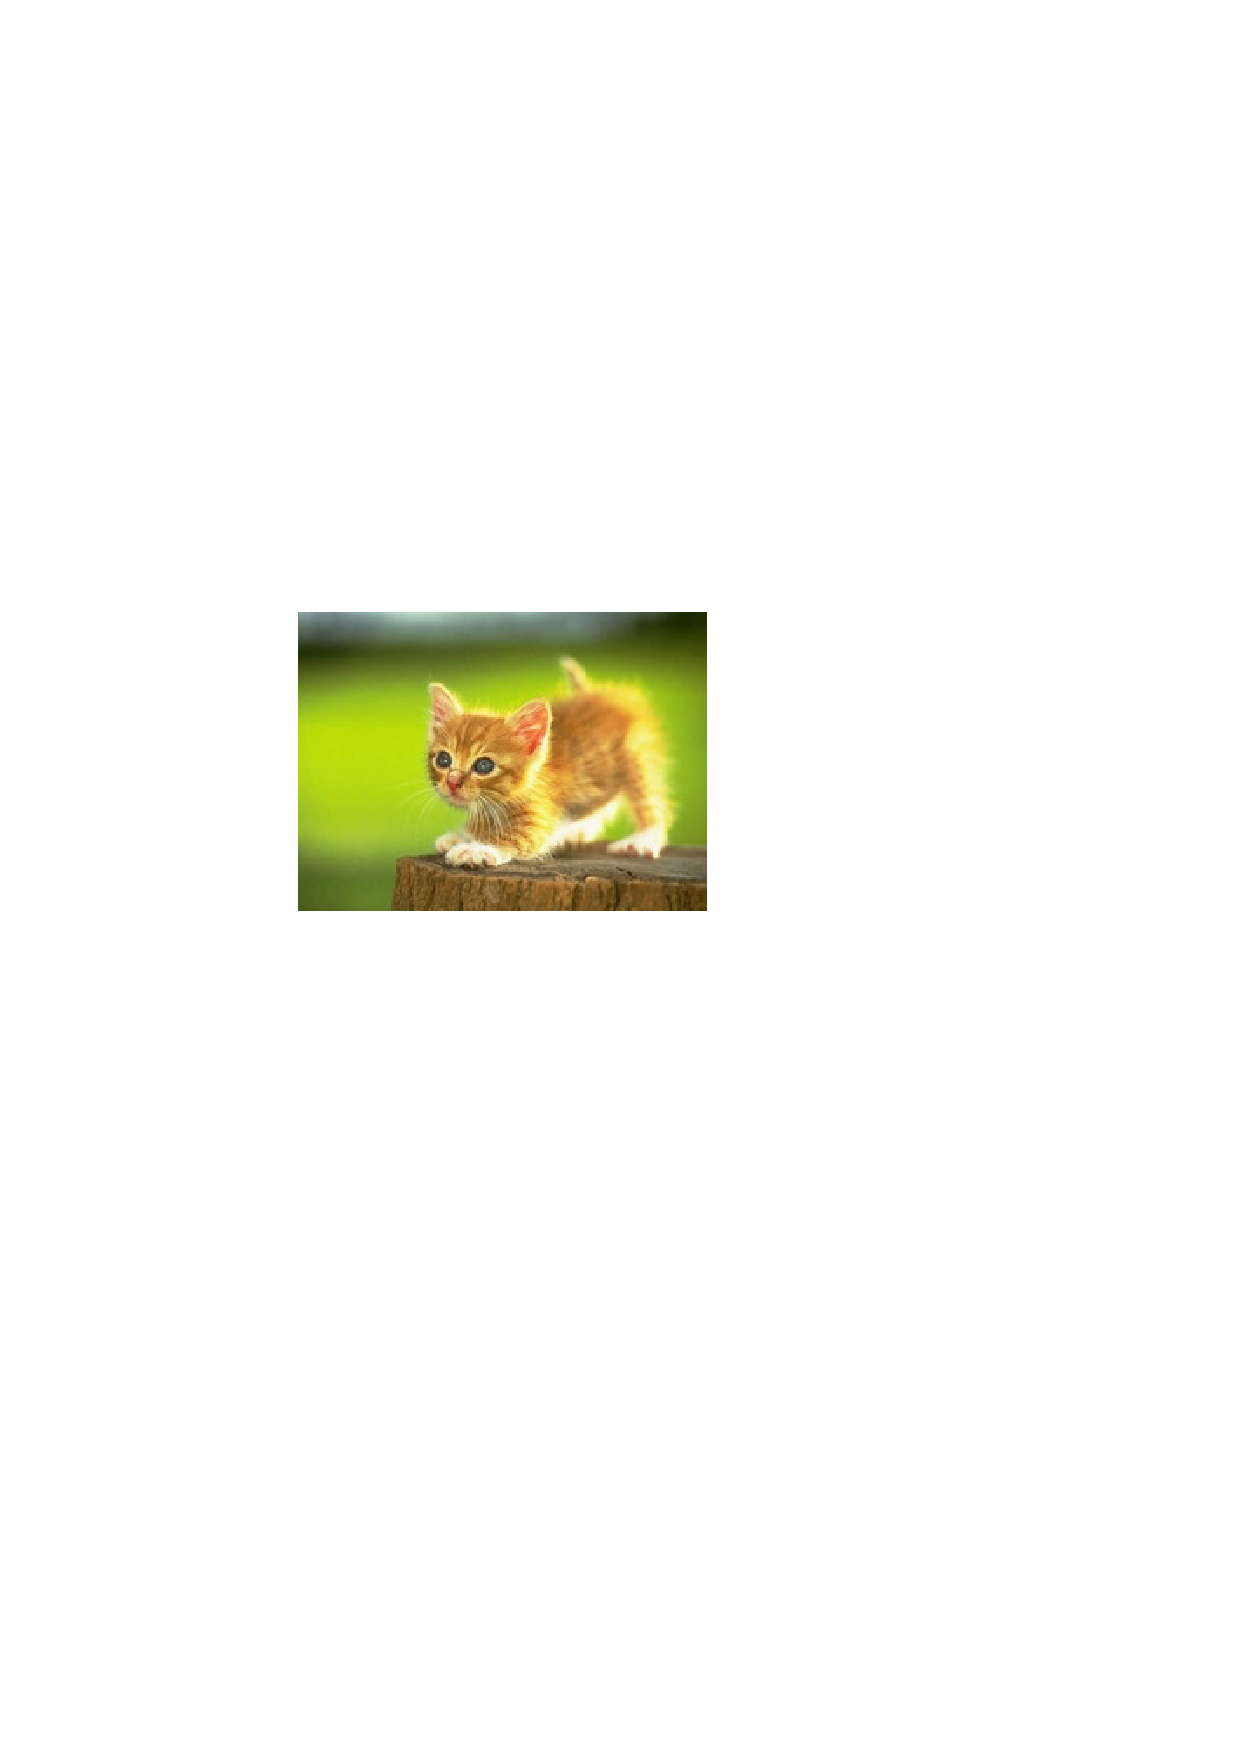
\includegraphics[width=.4\textwidth]{fig-example.pdf}
\caption{一个图片}\label{fig:1}
\end{figure}

\begin{figure}[!h]
\centering
  \begin{subfigure}[b]{0.3\textwidth}
  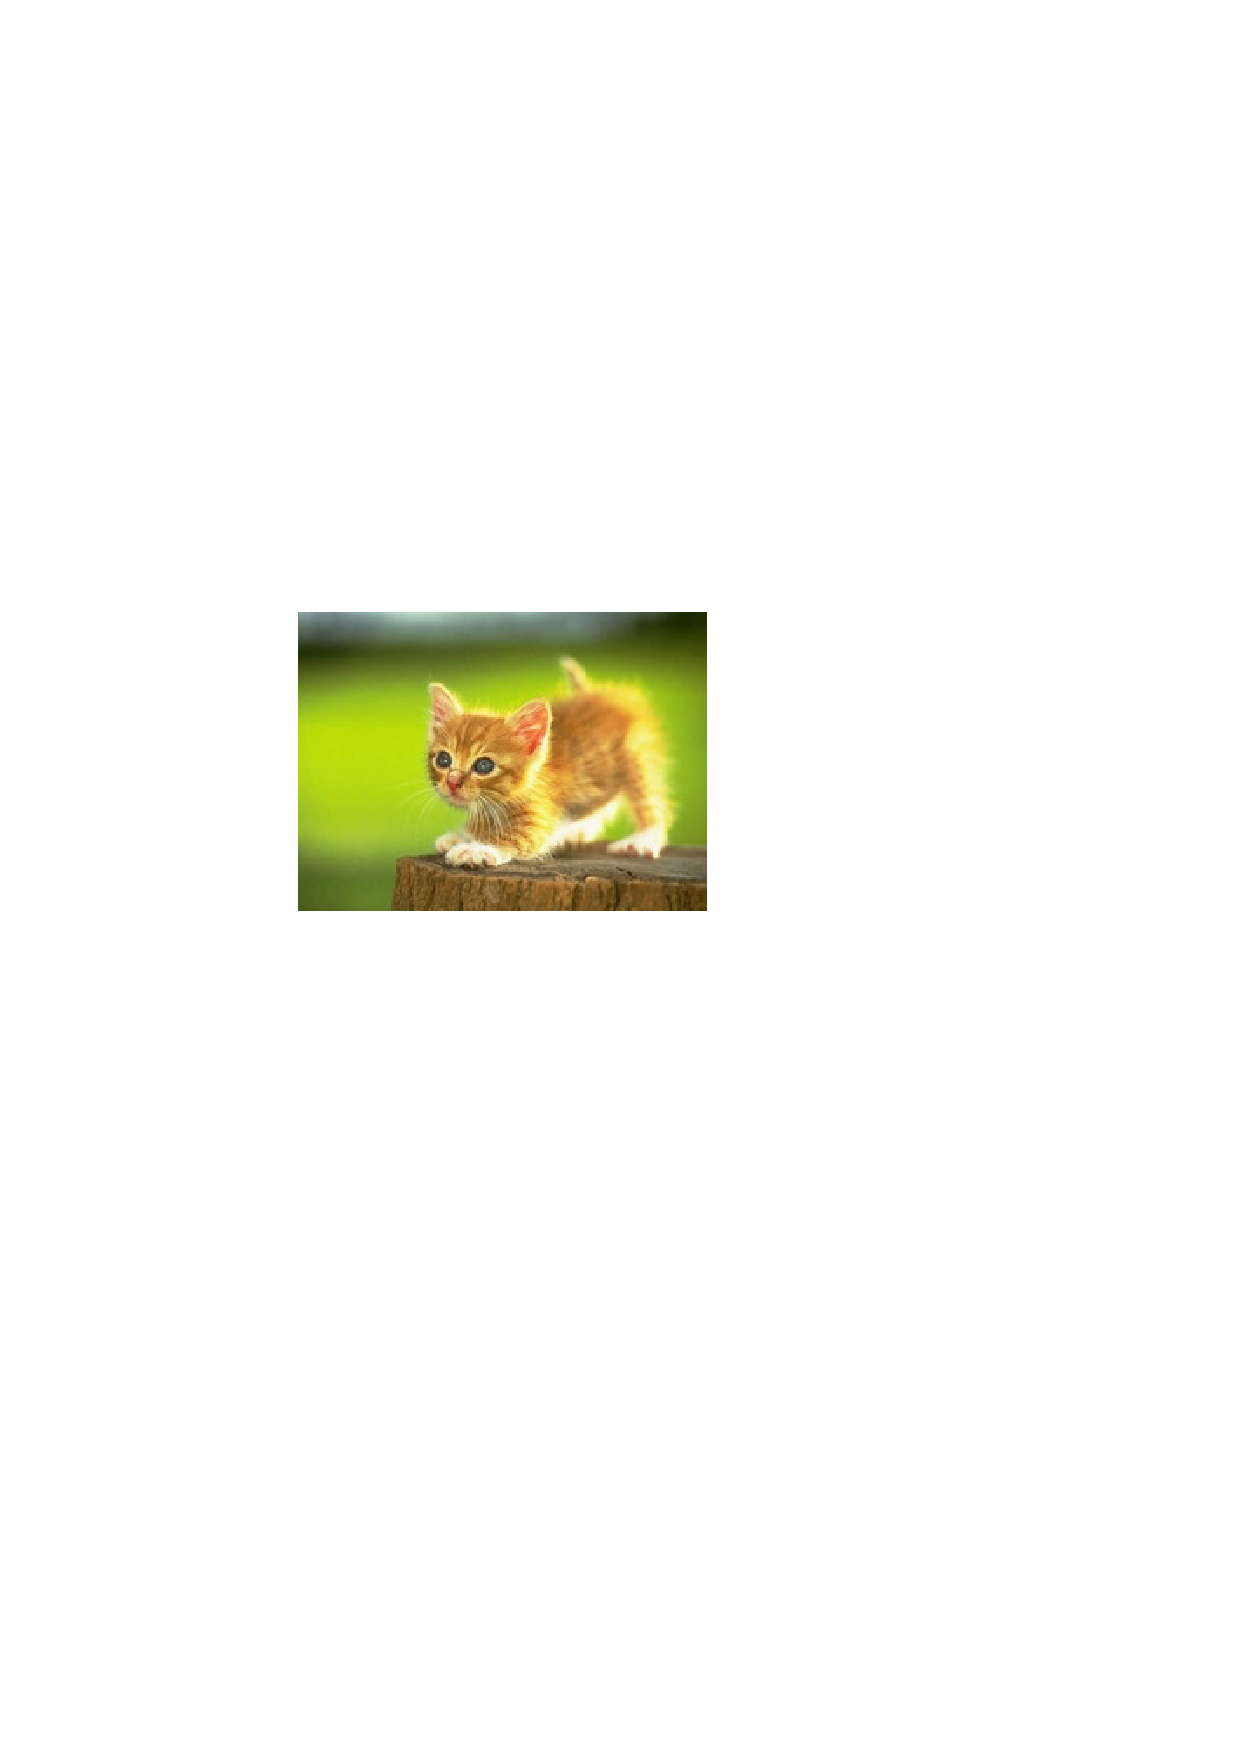
\includegraphics[width=\textwidth]{fig-example.pdf}
  \caption{图片1}\label{fig:2-1}
  \end{subfigure}
  ~
  \begin{subfigure}[b]{0.3\textwidth}
  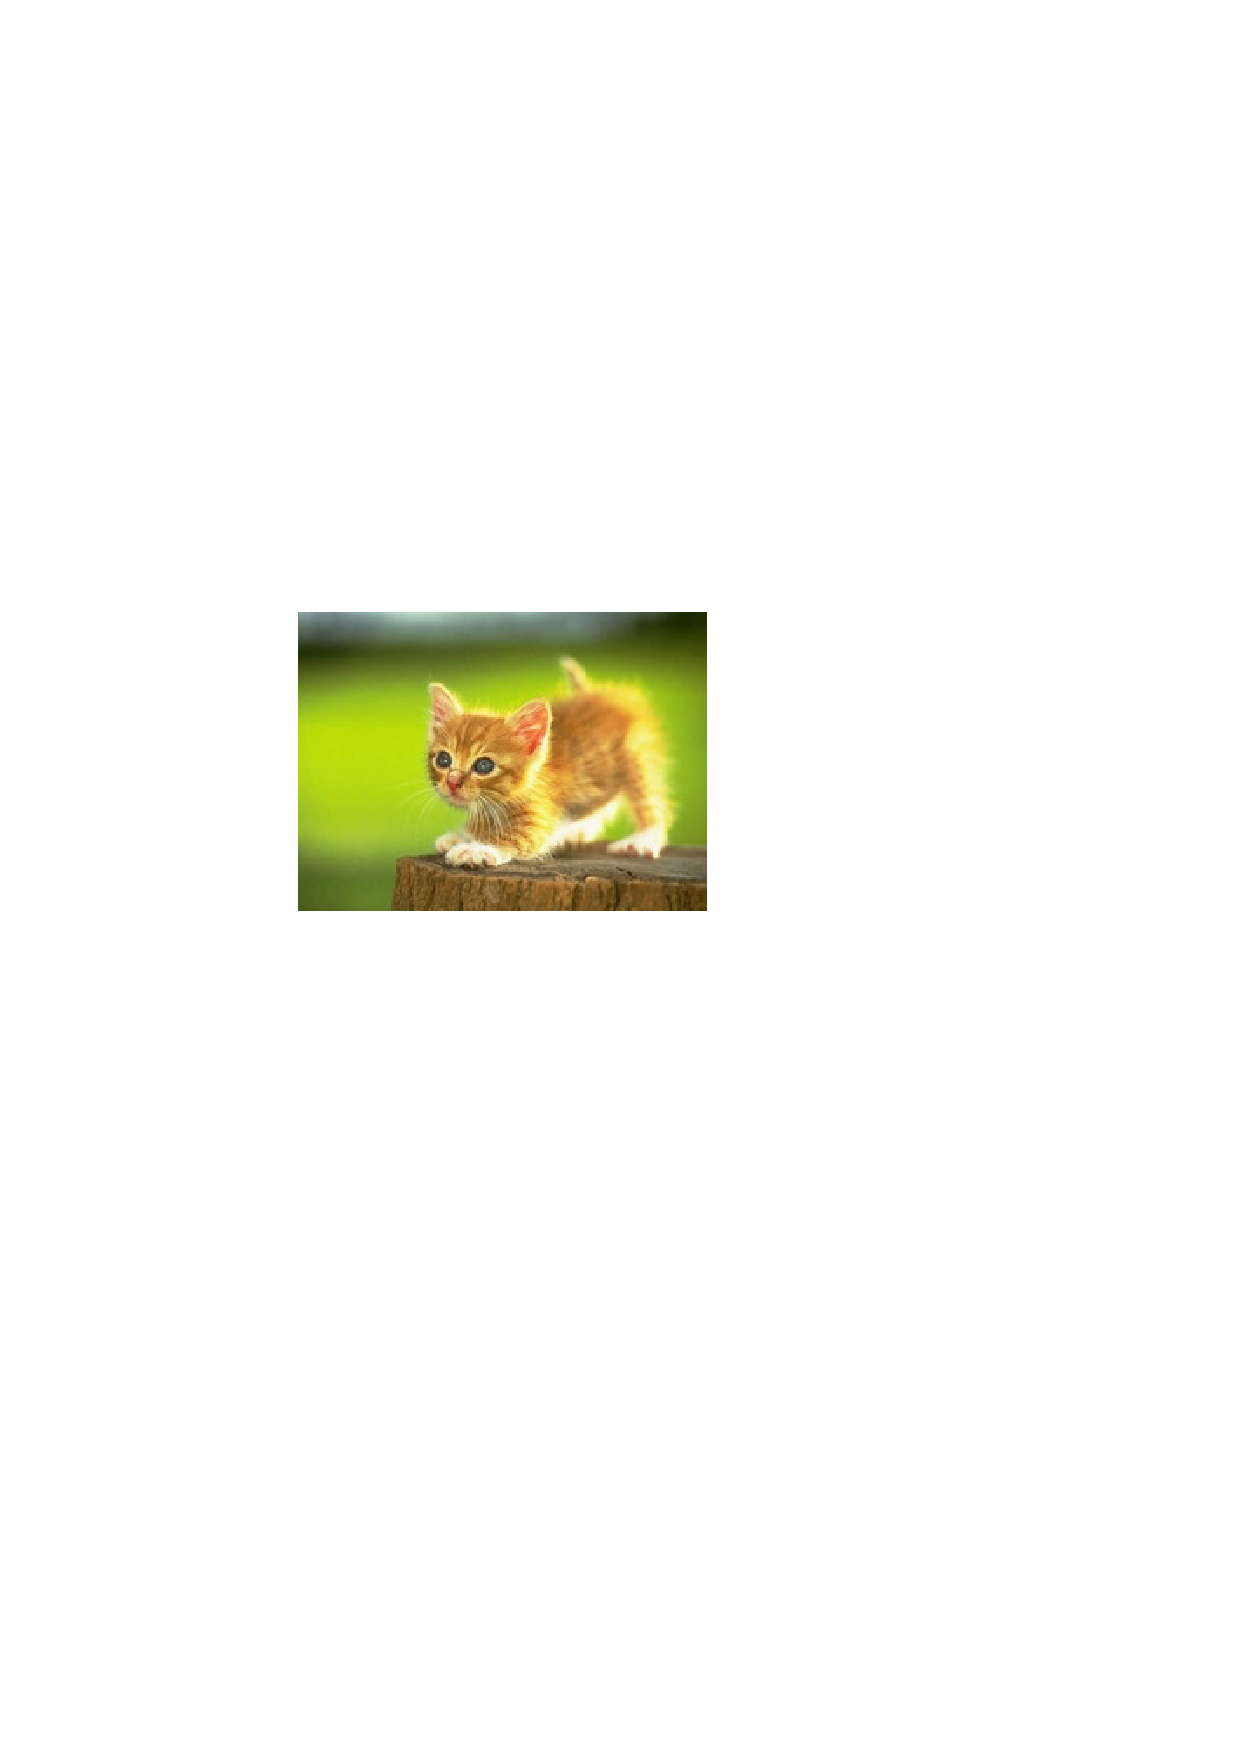
\includegraphics[width=\textwidth]{fig-example.pdf}
  \caption{图片2}\label{fig:2-2}
  \end{subfigure}
\caption{多个图片}\label{fig:2}
\end{figure}

\section{参考文献示例}
这是一篇中文参考文献\cite{TEXGURU99};这是一篇英文参考文献\cite{knuth};同时引用\cite{TEXGURU99,knuth}。

\section[\textbackslash{}autoref 测试]{\texttt{\textbackslash{}autoref} 测试}

\begin{description}
  \item[公式] \autoref{eq:1}
  \item[脚注] \autoref{footnote:1}
  \item[项] \autoref{item:1},\autoref{item:2},\autoref{item:3}
  \item[图] \autoref{fig:1}
  \item[表] \autoref{tab:1}
  \item[附录] \autoref{appendix:1}
  \item[章] \autoref{chapter:1}
  \item[小节] \autoref{sec:1},\autoref{sec:2},\autoref{sec:3}
  \item[算法] \autoref{alg:1},\autoref{alg_line:1}
  \item[证明环境] \autoref{def:1},\autoref{proposition:1},\autoref{axiom:1},\autoref{lemma:1},\autoref{theorem:1},\autoref{proof:1}
\end{description}


\backmatter

\begin{ack}
致谢正文。
\end{ack}

\bibliography{ref-example}

\appendix

\begin{publications}
    \item 论文1
    \item 论文2
\end{publications}

\chapter{这是一个附录}\label{appendix:1}
附录正文。

%</example-zh>
%<*example-en>
\chapter{Simple Test}\label{chapter:1}

\section{Level 1}\label{sec:1}
\subsection{Level 2}\label{sec:2}
\subsubsection{Level 3}\label{sec:3}
Content
\footnote{\label{footnote:1}A footnote.}

\section{Font}

Normal \textbf{Bold} \emph{Italic} \textsf{Sans}

The quick brown fox jumps over the lazy dog.

\section{Equation}

Single equation, see \autoref{eq:1}.
\begin{equation}
  c^2 = a^2 + b^2 \label{eq:1}
\end{equation}

Multi-equations, see \autoref{eq:2} and \autoref{eq:3}.

\begin{subequations}
\begin{equation}
  F = ma \label{eq:2}
\end{equation}
\begin{equation}
  E = mc^2 \label{eq:3}
\end{equation}
\end{subequations}

\section{List Environment}

\begin{enumerate}
    \item Level 1\label{item:1}
    \item Level 1
    \begin{enumerate}
        \item Level 2\label{item:2}
        \item Level 2
        \begin{enumerate}
            \item Level 3\label{item:3}
            \item Level 3
        \end{enumerate}
    \end{enumerate}
\end{enumerate}

\begin{description}
    \item[Discription]  Content
\end{description}

\chapter{Other Test}

\section{Code Highlight}

\begin{lstlisting}[language=python]
import os

def main():
    '''
    doc here
    '''
    print 'hello, world' # Abc
\end{lstlisting}

\section{Theorem}

\begin{definition}\label{def:1}
This is a definition.
\end{definition}
\begin{proposition}\label{proposition:1}
This is a proposition.
\end{proposition}
\begin{axiom}\label{axiom:1}
This is an axiom.
\end{axiom}
\begin{lemma}\label{lemma:1}
This is a lemma.
\end{lemma}
\begin{theorem}\label{theorem:1}
This is a theorem.
\end{theorem}
\begin{proof}\label{proof:1}
This is a proof.
\end{proof}

\section{Algorithm}

\begin{algorithm}[H]
\SetAlgoLined
\KwData{this text}
\KwResult{how to write algorithm with \LaTeX2e }
initialization\;\label{alg_line:1}
\While{not at end of this document}{
read current\;
\eIf{understand}{
go to next section\;
current section becomes this one\;
}{
go back to the beginning of current section\;
}
}
\caption{How to write algorithms}\label{alg:1}
\end{algorithm}

\section{Table}
See \autoref{tab:1}.

\begin{table}[!h]
\centering
\caption{A table}\label{tab:1}
\begin{tabular}{|c|c|}
\hline
a & b \\
\hline
c & d \\
\hline
\end{tabular}
\end{table}

\section{Figure}
See \autoref{fig:1}.Figure supports format in eps, png, pdf and so on. Multi-figures, see \autoref{fig:2}. Reference separately: \autoref{fig:2-1}, \autoref{fig:2-2}.

\begin{figure}[!h]
\centering
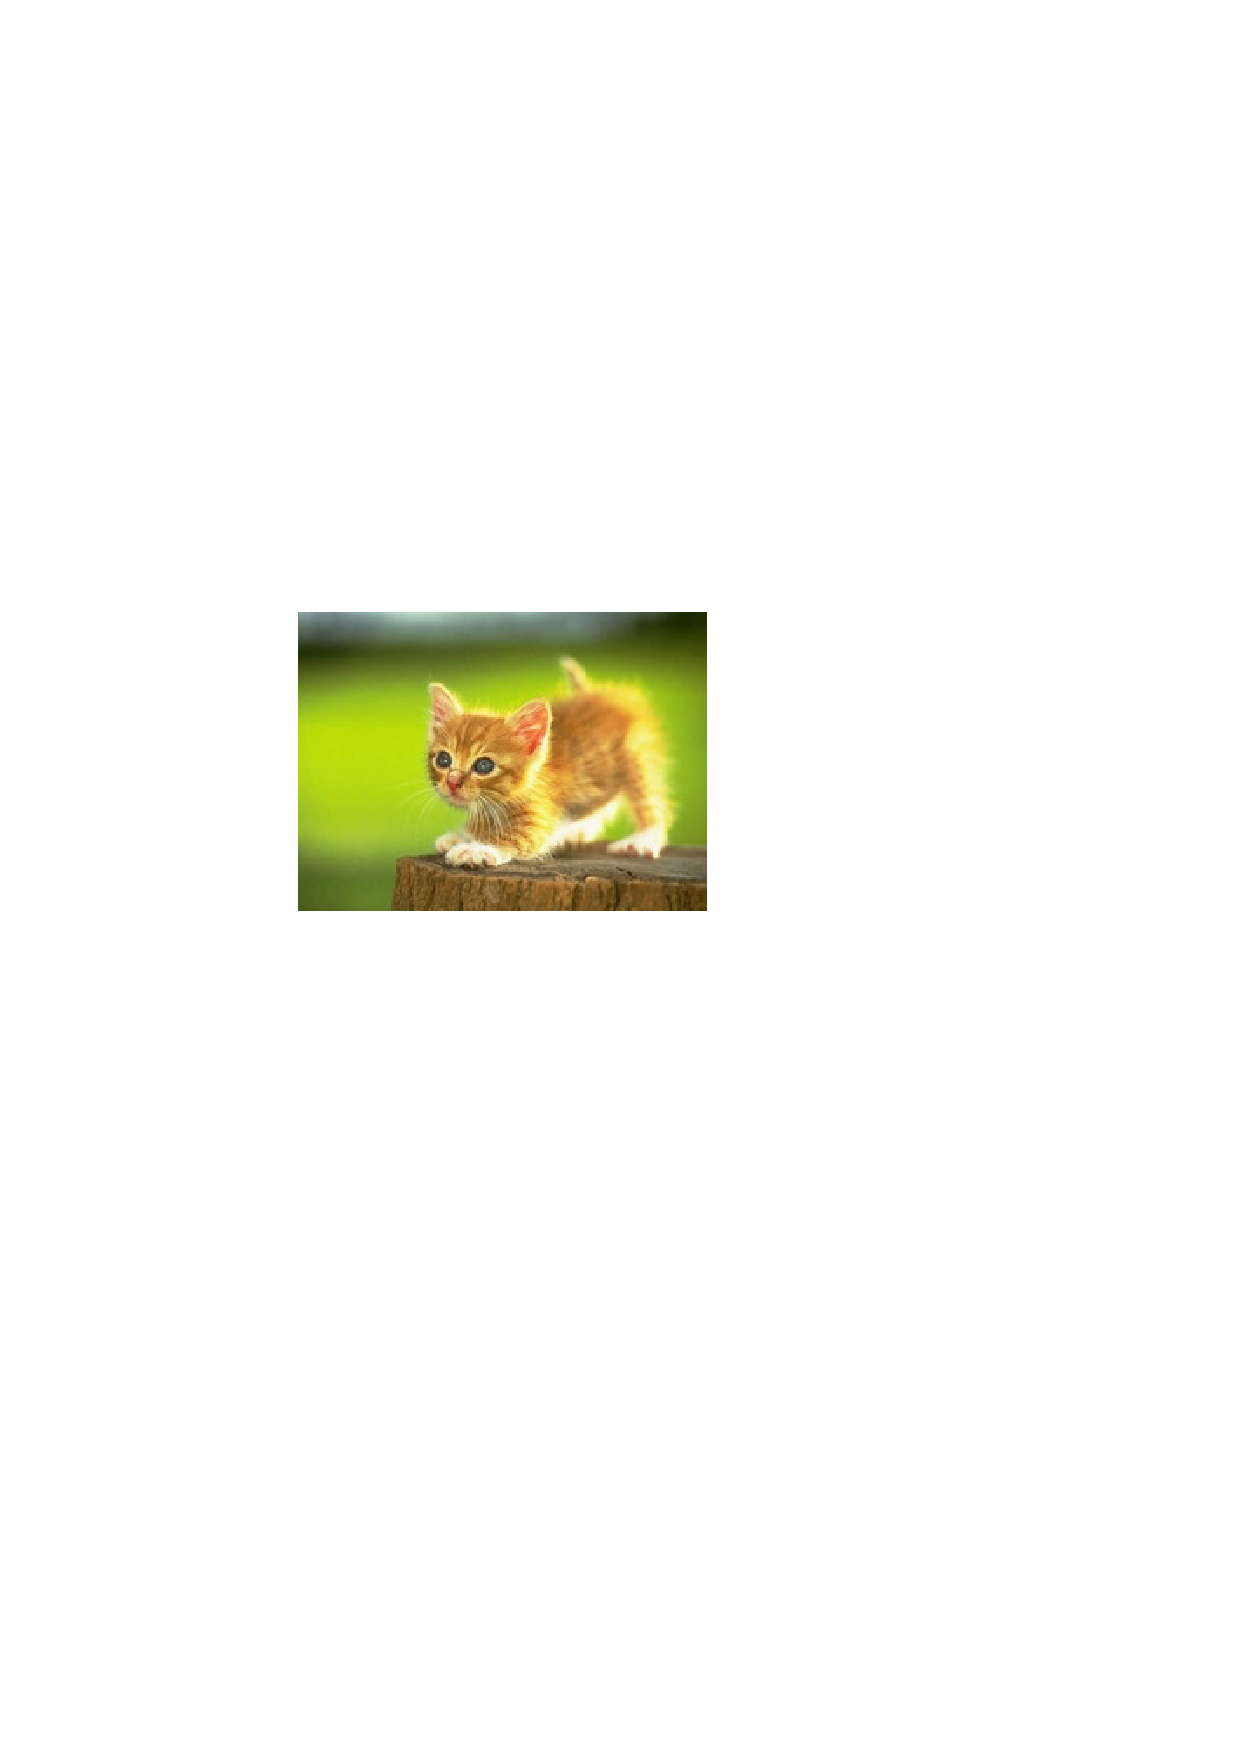
\includegraphics[width=.4\textwidth]{fig-example.pdf}
\caption{A figure}\label{fig:1}
\end{figure}

\begin{figure}[!h]
\centering
  \begin{subfigure}[b]{0.3\textwidth}
  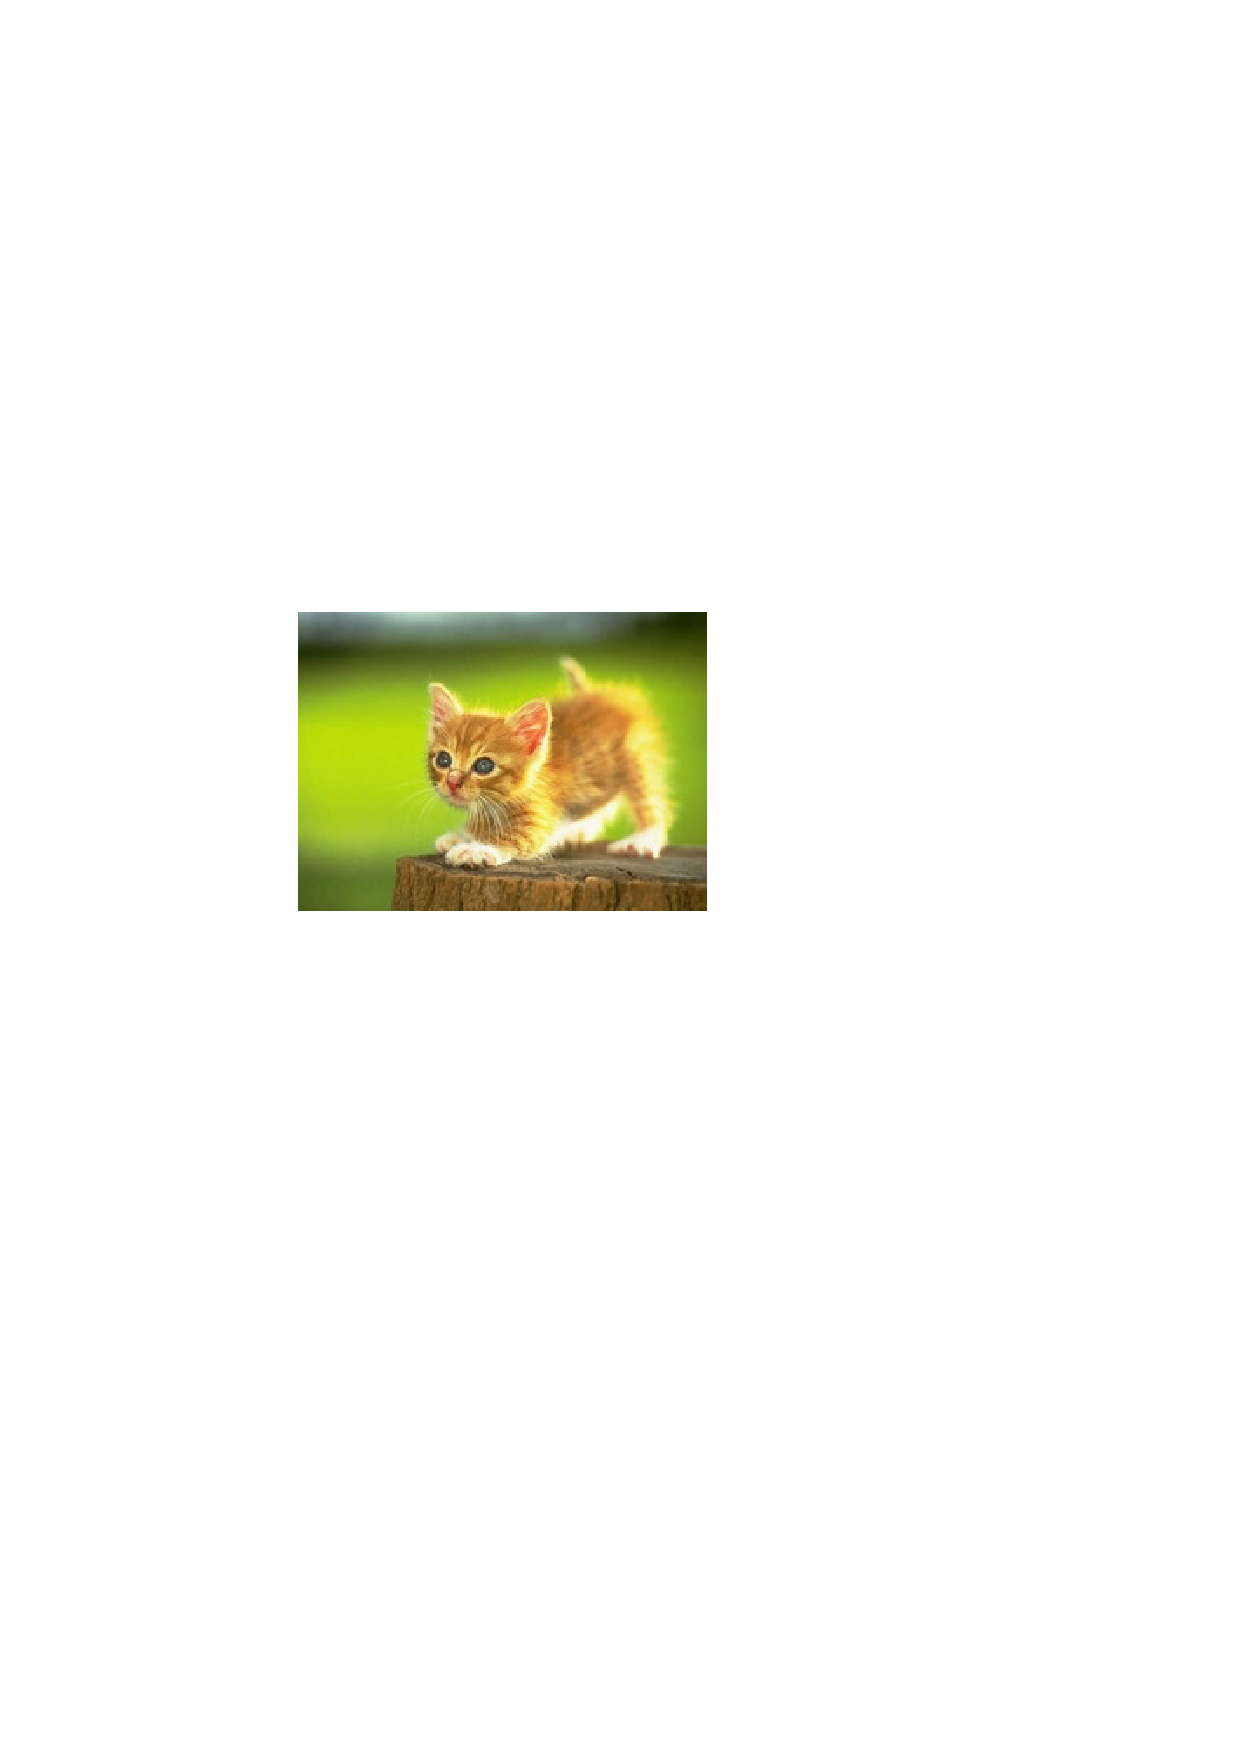
\includegraphics[width=\textwidth]{fig-example.pdf}
  \caption{Figure A}\label{fig:2-1}
  \end{subfigure}
  ~
  \begin{subfigure}[b]{0.3\textwidth}
  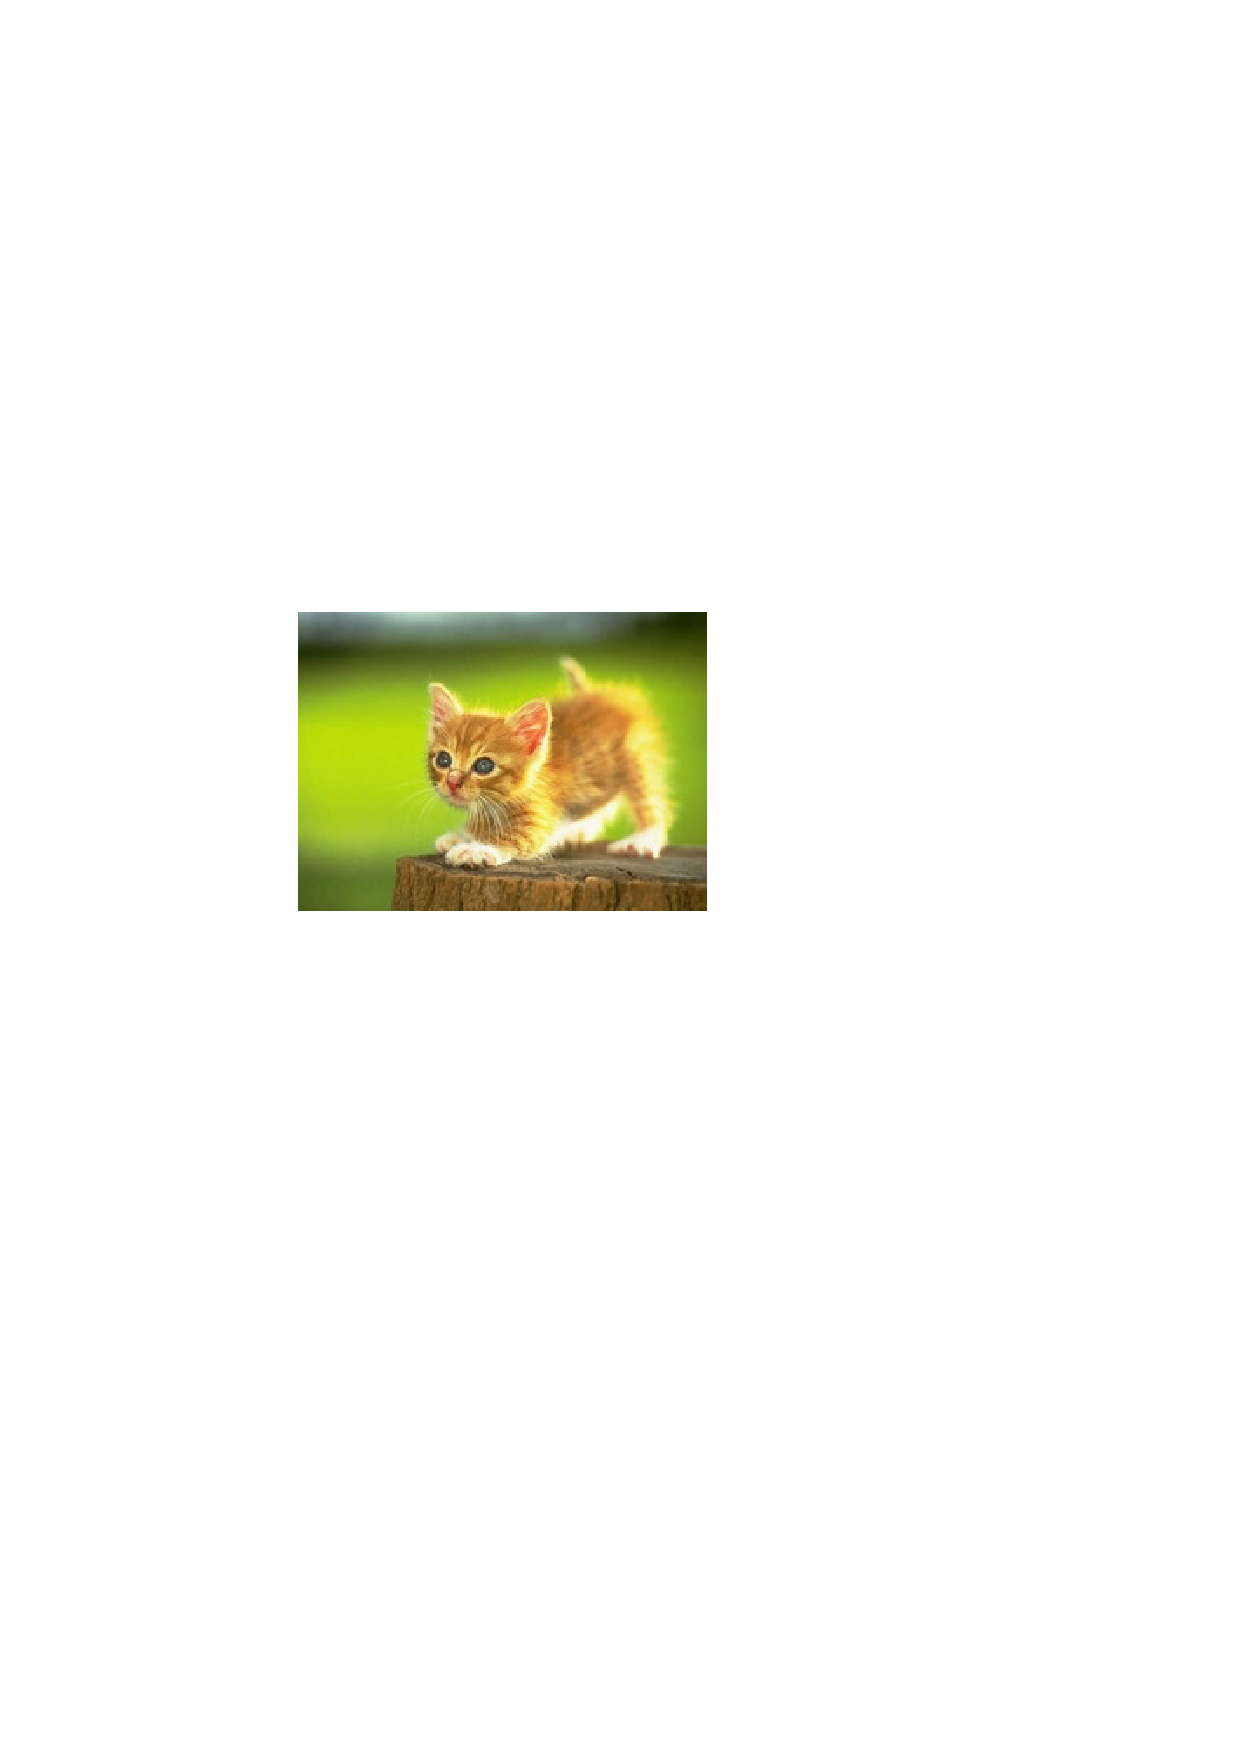
\includegraphics[width=\textwidth]{fig-example.pdf}
  \caption{Figure B}\label{fig:2-2}
  \end{subfigure}
\caption{Multi-figures}\label{fig:2}
\end{figure}

\section{Bibliography}
Cite one bib\cite{knuth}, cite two\cite{TEXGURU99,knuth}.

\section[\textbackslash{}autoref Test]{\texttt{\textbackslash{}autoref} Test}

\begin{description}
  \item[Equation] \autoref{eq:1}
  \item[Footnote] \autoref{footnote:1}
  \item[Item] \autoref{item:1},\autoref{item:2},\autoref{item:3}
  \item[Figure] \autoref{fig:1}
  \item[Table] \autoref{tab:1}
  \item[Appendix] \autoref{appendix:1}
  \item[Chapter] \autoref{chapter:1}
  \item[Section] \autoref{sec:1},\autoref{sec:2},\autoref{sec:3}
  \item[Algorithm] \autoref{alg:1},\autoref{alg_line:1}
  \item[Theorem] \autoref{def:1},\autoref{proposition:1},\autoref{axiom:1},\autoref{lemma:1},\autoref{theorem:1},\autoref{proof:1}
\end{description}

\backmatter

\begin{ack}
Acknowledge
\end{ack}

\bibliography{ref-example}

\appendix

\begin{publications}
    \item Thesis 1
    \item Thesis 2
\end{publications}

\chapter{This is an appendix}\label{appendix:1}
Content.

%</example-en>

\end{document}
%</example-zh|example-en>
%
%<*example-bib>
@BOOK{TEXGURU99,
  AUTHOR        = "{\TeX}Guru",
  TITLE         = "{\LaTeXe} Manual",
  YEAR          = "1999"
}

@BOOK{knuth,
  AUTHOR        = "{Donald E. Knuth}",
  TITLE         = "The \TeX{}book",
  publisher     = "Addison–Wesley Pub. Co.",
  address       = "MA",
  YEAR          = "1984"
}
%</example-bib>
%
% \fi
%
\endinput
